\graphicspath{{./04-Experimentale/images/}}

\chapter{Travaux expérimentaux}
\label{chap:experimental}
	Le milieu granulaire qui est étudié dans les travaux de cette thèse est un milieu constitué de grains de polystyrène. Les particules ont une taille moyenne de \SI{150}{\micro\meter} et leurs formes sont très irrégulières. Le comportement du polystyrène est décrit dans le paragraphe \ref{para03:PS}.
	\\Afin d'analyser la réponse mécanique du milieu à des conditions de compression multiaxiales, l'essai de compression triaxiale de révolution a été choisi. Avec cet essai, le milieu granulaire va être confiné de manière isotrope puis, dans le même temps, un déplacement selon l'axe de l'échantillon est imposé de manière à engendrer une compression axiale. Le dispositif est instrumenté au moyen de capteurs de déplacement et de force dans le but de mesurer la déformation globale de l'échantillon et de connaître les efforts auxquels l'ensemble de grains est soumis.
	\\Dans le but d'obtenir des informations concernant la microstructure du milieu granulaire, une technique d'imagerie 3D est mise en \oe{}uvre. Ainsi, la tomographie à rayons X va permettre d'obtenir un champ de densité du milieu mais également des champs de déplacements et de déformations. L'obtention des déplacements et des déformations avec l'imagerie 3D est rendue possible grâce aux méthodes de corrélation de volumes numérique.

\section{Essais de compression triaxiale de révolution}
	L’essai de compression triaxiale de révolution suit un principe opératoire classique pour obtenir un mode de sollicitation homogène au sein de l’échantillon. A ce titre, un essai mené de manière idéale permet de ne suivre qu'un seul chemin de chargement. Compte tenu du fait que les travaux de cette thèse intègrent une approche par simulation numérique, la mise en \oe{}uvre d’un essai homogène est d’un grand intérêt pour observer des conditions aux limites proches entre expérimentation et simulation. Pour cette raison le protocole décrit ci-dessous montrera les étapes qui permettront de réaliser au mieux ce type d’essai.
	\subsection{Matériel et protocole expérimentale}
		Les essais de compression triaxiale (cf. paragraphe \ref{para03:triax}) ont été menés sur différents échantillons de poudre de polystyrène. La figure \ref{fig04:triax} rappelle le principe de la compression triaxiale. Bien que les essais aient des caractéristiques différentes, le protocole expérimental est toujours le même et respecte les étapes suivantes, illustrées par la figure \ref{fig04:deroulement_essai}.
		\begin{figure}\centering
			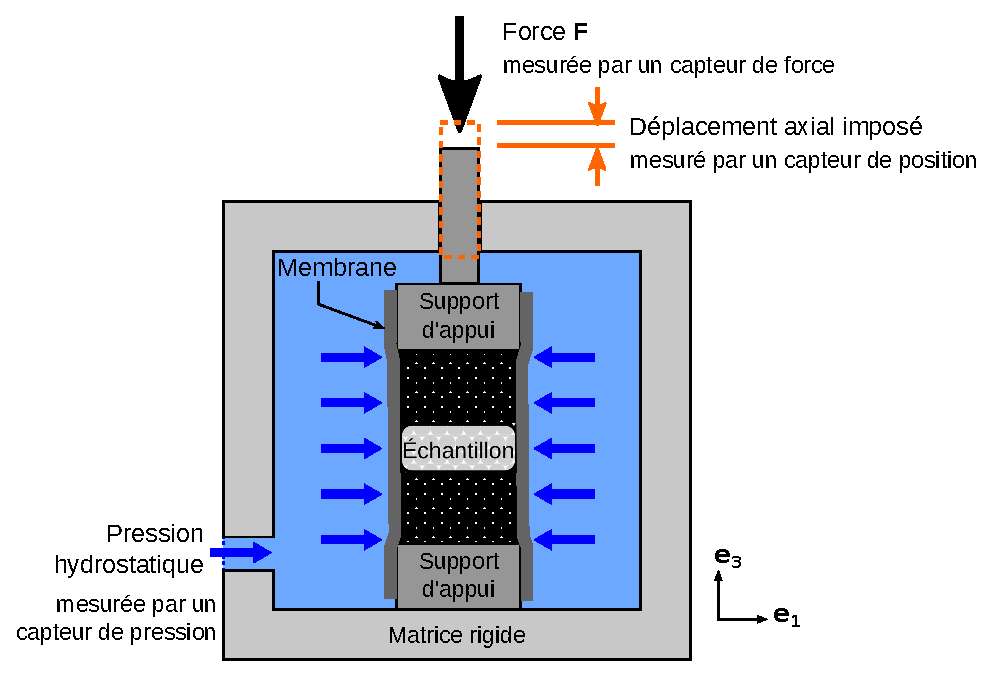
\includegraphics[scale=0.9]{../../03-Biblio/images/triax.eps}
			\caption{\label{fig04:triax}Principe de l'essai de compression triaxiale (cf. paragraphe \ref{para03:triax}).}
		\end{figure}
		\begin{figure}\centering
			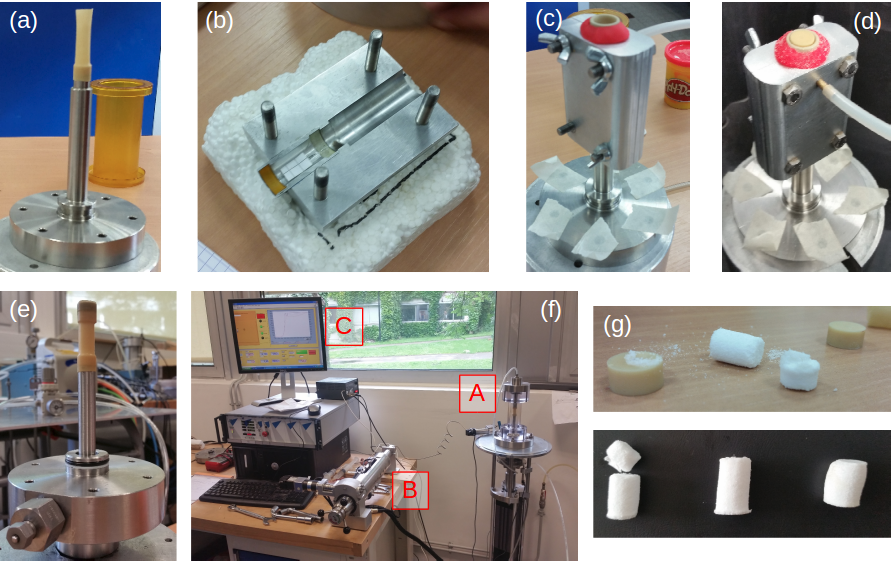
\includegraphics[width=1.\textwidth]{deroulement_essai.png}
			\caption{\label{fig04:deroulement_essai}Les différentes étapes de réalisation de la compression triaxiale de révolution.}
		\end{figure}
		\begin{description}
			\item[Figure \ref{fig04:deroulement_essai}-(a)] Une membrane étanche à l'eau en caoutchouc naturel, de forme cylindrique et de diamètre \SI{10}{\milli\meter}, d'épaisseur de paroi \SI{0.40}{\milli\meter} et de longueur \SI{50}{\milli\meter} est mise en place sur le poinçon supérieur du dispositif de compression et dont le diamètre est de \SI{12.5}{\milli\meter}. Une pièce en céramique percée est placée sur le support afin d'isoler la poudre du poinçon métallique et de laisser passer l'air dans l'échantillon. Cette pièce intermédiaire permet d'éviter la surexposition sur le détecteur de rayons X au niveau du poinçon métallique (le métal absorbe très significativement les rayons X par rapport au polystyrène). Laisser passer l'air dans l'échantillon permet de créer une dépression dans l'échantillon avant la mise en place définitive du dispositif.
			\item[Figure \ref{fig04:deroulement_essai}-(b)] Un moule de remplissage est ensuite utilisé afin de s'assurer de la géométrie cylindrique de l'échantillon et de faire en sorte que le diamètre de l'échantillon soit constant sur la hauteur et idéalement de \SI{10.2}{\milli\meter}. Un orifice dans le moule rigide permet de créer une dépression entre la membrane et le moule afin de forcer la membrane à se déformer pour épouser la forme du moule. Une feuille de papier est placée devant l'orifice pour diffuser les flux d'air et ne pas déformer de manière trop importante la membrane au niveau de l'orifice.
			\item[Figure \ref{fig04:deroulement_essai}-(c)] La seconde partie du moule est assemblée avec la première, la membrane est décalottée et de la pâte à modeler est placée pour assurer le maintien de la membrane et l'obstruction de l'air entre le moule et la membrane. Une pompe électrique Fisher Scientific FB70155 crée la dépression ($\approx$ \SI{20}{\kilo\pascal}) entre la membrane et le moule.
			\item[Figure \ref{fig04:deroulement_essai}-(d)] La membrane est remplie par pluviation de la manière la plus homogène possible. Une pièce en céramique (non percée) est placée sur la poudre puis, après avoir désactivé la pompe électrique, la membrane est placée sur cette céramique. La pompe électrique est ensuite branchée au niveau de la céramique percée afin de créer la dépression dans l'échantillon.
			\item[Figure \ref{fig04:deroulement_essai}-(e)] Le moule de remplissage est retiré délicatement. L'échantillon doit être bien droit. Tant que l'échantillon n'est pas plongé dans la cellule remplie d'eau et bien étanchéifiée, la dépression interne est maintenue.
			\item[Figure \ref{fig04:deroulement_essai}-(f)] L'échantillon et le support sur lequel il est fixé sont introduits dans la cellule de chargement en PMMA (polyméthacrylate de méthyle) qui est transparente aux rayons X et qui autorise un chargement hydrostatique maximal de \SI{7}{\mega\pascal}. La cellule est ensuite fixée sur le dispositif de chargement [A]. Une pompe hydraulique Sanchez Technologies VPSSH 6-700 [B] est saturée en eau afin de garantir une pression pouvant atteindre \SI{7}{\mega\pascal} pendant plusieurs jours. Enfin le système d'acquisition basé sur une interface Labview [C] est configuré en fonction des capteurs utilisés et permet le mouvement du moteur lorsque l'opérateur le décide ou de manière programmée. Sur la plateforme de chargement, sont présents : un capteur de force HBM C2 de \SI{5}{\kilo\newton} pour mesurer la charge axiale, un capteur de déplacement LVDT HBM WI de \SI{10}{\milli\meter} pour mesurer le déplacement axial. La mesure de la pression de confinement est faite par le capteur de pression intégré à la pompe hydraulique.
			\item[Figure \ref{fig04:deroulement_essai}-(g)] \`A la fin de l'essai, le chargement est stoppé, la pression de confinement est ramenée à la pression atmosphérique et l'échantillon est retiré de se membrane.
		\end{description}
		Le protocole expérimental présenté ci-dessus est resté invariant durant toute la période d'essais qui s'est déroulée dans une salle dont la température est régulée à \SI{20}{\celsius}. Différents essais ont été menés avec différents paramètres comme décrit dans la partie qui suit.
	\subsection{Campagne d'essais}
		Le chargement appliqué à l'échantillon est réalisé par paliers de manière à stopper la déformation de l'échantillon pendant l'acquisition (scan) d'une image 3D. En raison des capacités du tomographe, de la taille de l'échantillon et de la réponse viscoélastique de l'échantillon, le temps de scan varie entre \SI{2}{\hour} et \SI{4}{\hour}.
		\\La figure \ref{fig04:geometries_membrane} montre l'évolution de l'échantillon dans sa membrane au cours du chargement. La déformation maximale appliquée à l'échantillon est de 0.25 (déformation logarithmique axiale). Au-delà de cette valeur, l'hétérogénéité du champ de déformation se traduit presque systématiquement par un désaxement important de l'échantillon (dont on peut voir le début sur la figure \ref{fig04:geometries_membrane}-(b)).
		\\En tenant compte de l'ensemble de ces contraintes, la durée des essais réalisés est comprise entre \SI{40}{\hour} et \SI{50}{\hour}.
		\begin{figure}\centering
			~\hfill
			\subfloat[]{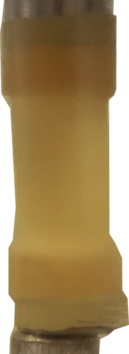
\includegraphics[width=0.15\textwidth]{00_membrane_small.png}}\hfill
			\subfloat[]{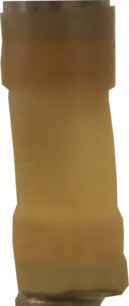
\includegraphics[width=0.15\textwidth]{01_membrane_small.png}}\hfill
			\subfloat[]{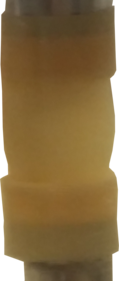
\includegraphics[width=0.15\textwidth]{02_membrane_small.png}}\hfill~
			\caption{\label{fig04:geometries_membrane}Déformation d'un échantillon dans sa membrane en cours de compression avec une pression de confinement de \SI{1}{\mega\pascal}: échantillon (a) avant compression, (b) en milieu d'essai [déformation logarithmique axiale de \num{0.15}] et (c) en fin d'essai [déformation axiale de \num{0.25}].}
		\end{figure}
		\\Trois essais de compression triaxiale de révolution ont été menés au sein du tomographe du laboratoire 3SR. Les essais ont été menés à trois pressions de confinement différentes : \SI{1}{\mega\pascal}, \SI{2}{\mega\pascal} et \SI{7}{\mega\pascal}. Lorsque le piston se déplace, la vitesse axiale de \SI{2}{\micro\meter\per\second} est la même pour l'ensemble des essais.
		\\La figure \ref{fig04:courbes_manip_temps} permet d'observer l'évolution de l'avancée du piston et la mesure de la force sur celui-ci au cours du temps. Les paliers de chargement entre chaque arrêt correspondent à des avancées du piston de quelques centaines de micromètres. Le pilotage en déplacement est facilement observable sur la figure \ref{fig04:courbes_manip_temps} -(a). La figure \ref{fig04:courbes_manip_temps} -(b) permet d'observer, quant à elle, la force axiale appliquée par le piston à l'échantillon. Les temps de scan sont de l'ordre de deux heures et, pendant cette durée, l'échantillon oppose une réponse viscoélastique au déplacement axial et à la contrainte de confinement imposés, qui se traduit notamment par une relaxation de la contrainte axiale. Dans le but d'acquérir les images les plus nettes possible et de s'assurer que la microstructure de l'échantillon reste stable pendant le scan, il a été choisi d'attendre un certain temps entre l'arrêt du chargement et le commencement du scan de tomographie afin que le relâchement de contrainte soit relativement léger sur le temps de scan. Ce temps de latence va de deux heures pour les premiers états de chargement jusqu'à plus de quatre heures pour les états de chargement les plus élevés.
		\begin{figure}\centering
			\subfloat[]{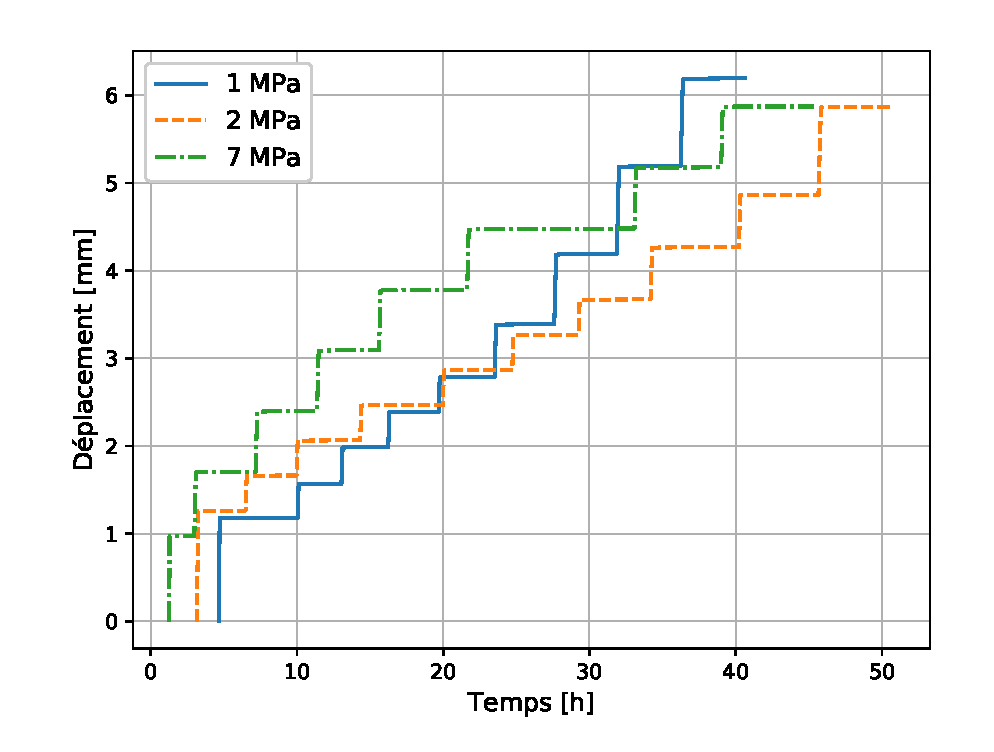
\includegraphics[width=0.49\textwidth]{displacement_time.eps}}\hfill
			\subfloat[]{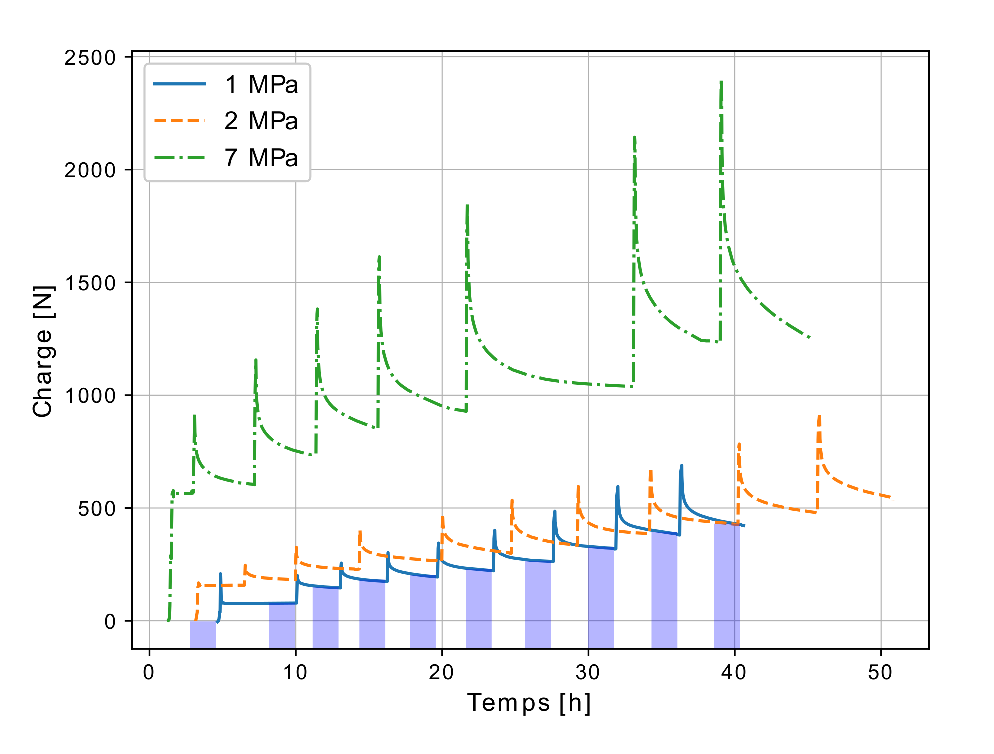
\includegraphics[width=0.49\textwidth]{load_time_scanTimes.eps}}
			\caption{\label{fig04:courbes_manip_temps}Courbes (a) du pilotage en déplacement du piston et (b) de la force mesurée sur le piston par rapport au temps pour l'ensemble des essais réalisés. Les zones en transparence bleue indiquent les temps de scan de tomographie pour l'essai dont la pression de confinement est \SI{1}{\mega\pascal}. Comme dans la suite, les essais sont triés par pression de confinement.}
		\end{figure}
		\\Il est observable sur la figure \ref{fig04:courbes_manip_temps} -(b) que l'échantillon dont le confinement est de \SI{1}{\mega\pascal} subit une pression de surconsolidation de \SI{2}{\mega\pascal}. Pour cela, la pression de confinement est augmentée jusqu'à cette valeur puis elle est ensuite diminuée jusqu'à la pression de confinement de \SI{1}{\mega\pascal} attendue pour l'essai.
	\subsection{Mesure des propriétés mécaniques des échantillons}
		Afin de comprendre la réponse globale de l'échantillon à la compression triaxiale, des calculs de contrainte et de déformation sont menés à partir des mesures de force et déplacement.
		\\Pour cela, des mesures de l'échantillon sont prises avant commencement du chargement par l'intermédiaire des images de tomographie. En effet, connaissant la taille des voxels, il est tout à fait possible de connaître la taille d'une structure en comptant le nombre de voxel selon la direction de la distance mesurée. L'échantillon est considéré à géométrie cylindrique parfaite (ce qui est relativement bien vérifié par l'observation des images de tomographie). Les mesures prises sont celle du diamètre de l'échantillon et de sa hauteur. En ce qui concerne le diamètre, plusieurs mesures sont faites sur la hauteur de l'échantillon et une valeur moyenne est choisie. Les mesures pour chacun des trois essais réalisés dans cette thèse sont présentées sur le tableau \ref{tab04:mesures_echantillons}.
		\begin{table}\centering
			\begin{tabular}{c@{\hspace{10mm}}c@{\hspace{10mm}}c}
				\hline
				Confinement & Diamètre [\si{\milli\meter}] & Hauteur [\si{\milli\meter}] \\\hline
				\SI{1}{\mega\pascal} & \num{10.10} & \num{21.30} \\
				\SI{2}{\mega\pascal} & \num{10.00} & \num{23.30} \\
				\SI{7}{\mega\pascal} & \num{10.15} & \num{22.70} \\\hline
			\end{tabular}
			\caption{\label{tab04:mesures_echantillons}Mesures des dimensions des échantillons.}
		\end{table}
		\\On fait l'hypothèse de l'homogénéité des essais. Alors, une méthode de calcul des contraintes ramenées à la surface initiale et déformations logarithmiques dans l'échantillon est de considérer la géométrie initiale de l'échantillon et la conservation de la géométrie cylindrique. Si cette dernière hypothèse s'avère vérifiée pour les petites déformations, elle n'est pas vérifiée lorsque la déformation atteint un niveau relativement élevé (cf. photographie du bas sur la figure \ref{fig04:deroulement_essai} -(g) et figure \ref{fig04:geometries_membrane}-(c)). Si $D_0$ est le diamètre initial de l'échantillon, $h_0$ sa hauteur initiale, $\Delta h$ le déplacement du piston par rapport à sa position initiale et $F$ la force mesurée par la capteur de force sur le piston, alors la contrainte axiale est définie selon l'équation (\ref{eq04:contrainte_echantillon}) et la déformation logarithmique axiale par l'équation (\ref{eq04:defo_echantillon}).
		\begin{equation}\label{eq04:contrainte_echantillon}
			\sigma_a = F \times \cfrac{4}{\pi D_0^2}
		\end{equation}
		\begin{equation}\label{eq04:defo_echantillon}
			\varepsilon_a = \ln\cfrac{h_0+\Delta h}{h_0}
		\end{equation}
		\`A partir de ces équations, il est possible d'utiliser les données présentées sur les graphes de la figure \ref{fig04:courbes_manip_temps} pour obtenir les courbes de contraintes-déformations présentées sur la figure \ref{fig04:courbes_manip_contrainte_defo}. Sur cette figure, la déformation axiale n'est pas mesurée lors de la mise sous pression de confinement puisque le piston reste immobile durant cette étape. Pour cette raison, les courbes ne sont valables qu'à partir du moment où le piston vient en contact de l'échantillon après la mise en confinement. Seule les parties valables des courbes sont tracées, ce qui explique l'absence d'information entre la déformation nulle et celle en début de courbe.
		\begin{figure}\centering
			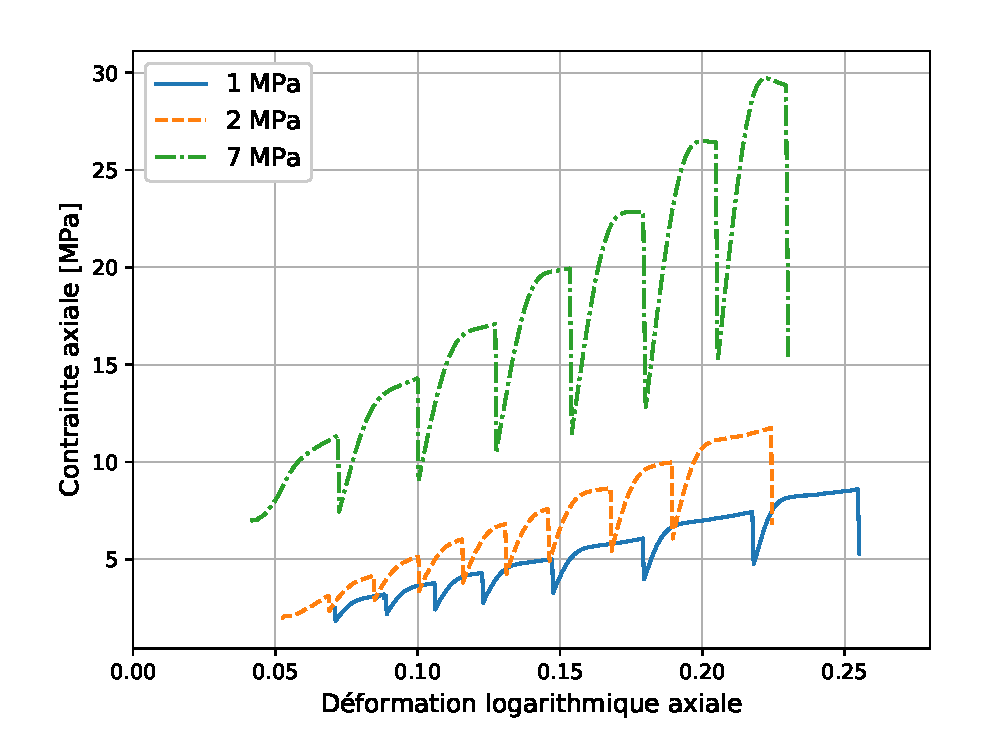
\includegraphics[width=0.7\linewidth]{stress_strain.eps}
			\caption{\label{fig04:courbes_manip_contrainte_defo}Courbes des contraintes-déformations de l'échantillon suivant la direction axiale du chargement.}
		\end{figure}
		\\L’évolution de la réponse mécanique au cours du temps permet de visualiser un comportement visco-élastique du milieu. Le comportement mécanique de l’échantillon conserve ce caractère visco-élastique jusqu’aux plus forts états de compression. Il est difficile dans cette réponse globale issue des capteurs de faire la part de la réponse mécanique de la cellule. La conception de la presse participant par exemple au frottement entre support et grains ou encore piston et support d’échantillon. Les courbes présentées sur les figures \ref{fig04:courbes_manip_temps}-(b) et \ref{fig04:courbes_manip_contrainte_defo} montrent cet effet visqueux par la relaxation de l'effort, et donc de la contrainte, lorsque la cinématique est figée. Lorsque le chargement axial reprend, après chaque arrêt du piston, la vitesse de déplacement du piston passe de manière quasi-instantanée d'une valeur nulle à une valeur de \SI{2}{\micro\meter\per\second} : cela engendre un ressaut de l'effort et de la contrainte à chaque reprise du chargement axial comme le montre les courbes.
		\\Il est observé également, par comparaison des courbes pour les trois valeurs de confinement, que la contrainte axiale est d'autant plus grande que la pression de confinement est grande pour des amplitudes de chargement fixées.
	\subsection{Essais hors tomographe}
		La compression de l'échantillon est menée en présence régulière d'un rayonnement X. Puisque la matière interagit aux rayons électromagnétiques de haute énergie, il est possible que la présence des rayons X modifie le comportement de l'échantillon si les rayons produits par le tomographe ont une énergie trop élevée. Afin de vérifier cette possibilité, des essais semblables à ceux menés au sein du tomographe ont été menés en dehors de la cabine d'exposition aux rayons X. La vitesse de sollicitation est toujours de \SI[per-mode=symbol]{2}{\micro\meter\per\second}. Les courbes contraintes-déformations de ces essais sont présentés sur la figure \ref{fig04:courbes_in_out}. Les courbes sur le graphe de gauche sont obtenues pour des pressions de confinement de \SI{250}{\kilo\pascal}, \SI{500}{\kilo\pascal}, \SI{1}{\mega\pascal}, \SI{2}{\mega\pascal}, \SI{4}{\mega\pascal} et \SI{7}{\mega\pascal}. Celles du graphe de droite sont les mêmes courbes (en traits pointillés) pour les pressions de confinement de \SI{1}{\mega\pascal}, \SI{2}{\mega\pascal} et \SI{7}{\mega\pascal} en présence des courbes (en traits continus) issues des essais menés dans le tomographe (essais \textit{in-situ}).
		\begin{figure}\centering
			\subfloat{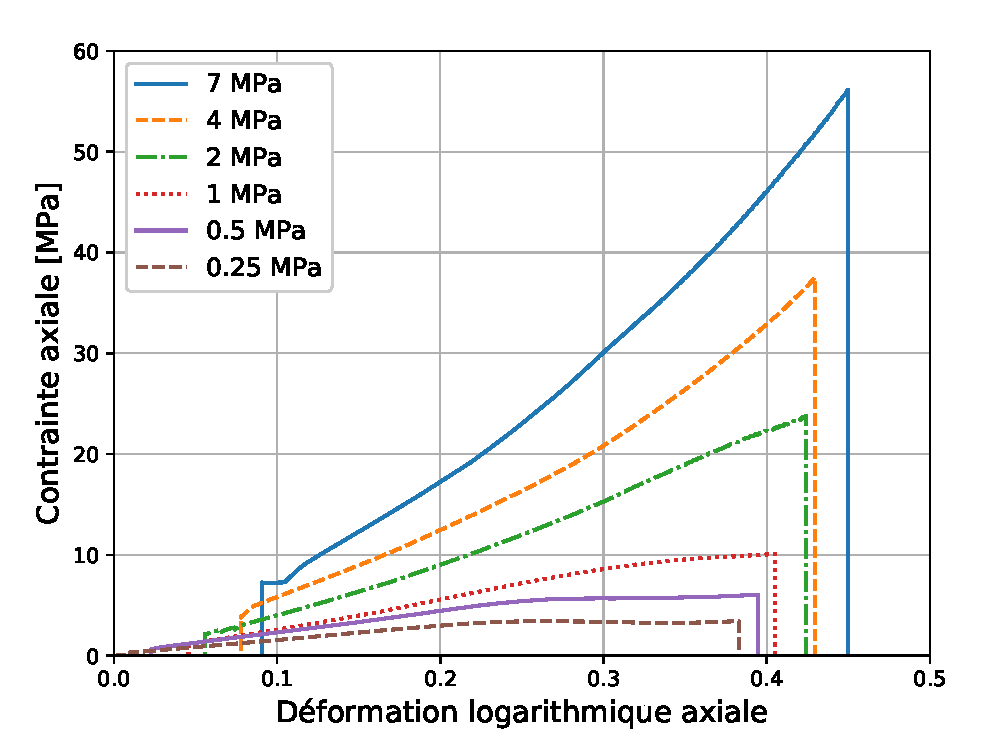
\includegraphics[width=.48\linewidth]{PS_stress-strain.eps}}\hfill
			\subfloat{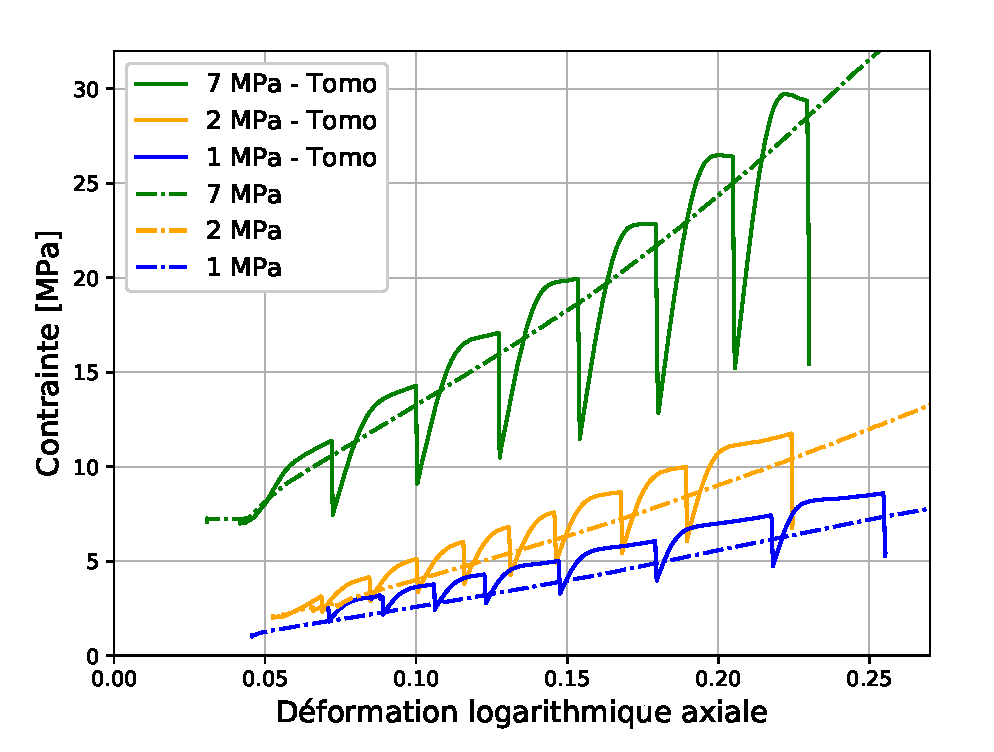
\includegraphics[width=.48\linewidth]{PS_in-out_stress-strain.eps}}
			\caption{\label{fig04:courbes_in_out}Courbes des contraintes-déformations pour (a) des essais de compression triaxiale à différentes pressions de confinement et sans interruption et (b) comparaison des essais menés dans le tomographe avec les mêmes essais menés en dehors.}
		\end{figure}
		Il est observé que dans les essais interrompus, la remise en charge (caractérisée par la fait que la vitesse de chargement imposée passe brusquement de \num{0} à \SI[per-mode=symbol]{2}{\micro\meter\per\second}), se traduit par un pic de contrainte jusqu'à une valeur supérieure à la contrainte obtenue pour le chargement monotone (sans interruption) pour la même déformation imposée. Cet effet est caractéristique du comportement viscoélastique et est observé notamment dans les essais de relaxation suite à un échelon en déformation. Il résulte du fait que le temps caractéristique de relaxation de l'échantillon (ou plutôt, de l'ensemble du dispositif incluant en particulier la cellule) est relativement faible par rapport à la vitesse de chargement. On voit également que le comportement à la remise en charge varie au cours du chargement, ce qui traduit la non-linéarité du système.
		\\L'analyse des graphes permet de constater, en particulier pour les pressions de confinement les plus faibles, que les courbes issues des essais ininterrompus semblent montrer une contrainte inférieure  à celles de la courbe maîtresse des essais interrompus. Plusieurs raisons peuvent être imaginées pour expliquer cette différence. Cet effet peut être rattaché à un phénomène mis en jeu lors de l'exposition du milieu granulaire aux rayons X. De plus, la précision de mesure des dimensions de l'échantillon est bien inférieure sur ces essais puisque la mesure au pied à coulisse permet une précision de l'ordre de \SI{0.02}{\milli\meter} alors que les images de tomographie permettent une précision inférieure à \SI{0.01}{\milli\meter}. Le rapport d'élancement de l'échantillon (rapport entre longueur et diamètre) avant essai est également un paramètre à prendre en compte. En ce qui concerne les essais hors tomographe, pour les pressions de confinement de \SI{1}{\mega\pascal}, \SI{2}{\mega\pascal} et \SI{7}{\mega\pascal}, les rapports d'élancement sont respectivement de \num{2.12}, \num{2.19} et \num{2.18}. Les essais, pour les mêmes pression de confinement, menés dans le tomographe sont réalisés sur des échantillons dont les rapports d'élancement sont de \num{2.11}, \num{2.33} et \num{2.24}. Une autre raison qui peut expliquer cette différence dans la mesure des contraintes est la condition de stockage des grains. En effet, les essais menés en dehors du tomographe ont été réalisés plusieurs mois après les essais menés dans le tomographe. Durant ces quelques mois, la poudre a été stockée à l'abri de la lumière, dans une salle dont la température est régulée mais dont l'humidité ne l'est pas. Il est donc possible que les propriétés des grains de polystyrène aient changées durant le temps de stockage par effet du vieillissement naturel. Enfin, les essais menés en dehors du tomographe sont réalisés sans interruptions, et donc ne subissent pas les mêmes contraintes de fluage et de relaxation.

\section{Tomographie à rayons X}\label{para04:tomo}
	\subsection{Matériel et protocole expérimental}
		Les scans sont réalisés par le microtomographe du laboratoire 3SR fabriqué par RX-Solutions (Annecy), avec une source Hamamatsu L12161-07 et un panneau de détection plat Varian.
		\\La figure \ref{fig04:manip_tomo} présente le dispositif d'acquisition avec le système de chargement tels qu'ils sont dans les expériences présentés dans ces travaux. On remarque que la distance entre la source et l'échantillon est minimale. Cette distance est réglable et permet de définir la résolution de l'image, déterminée en micromètre et correspondant à la taille d'un côté d'un voxel. Plus la distance est courte, meilleure est la résolution. Dans ces travaux, la résolution de \SI{9}{\micro\meter} est finalement la résolution maximale pour le dispositif du laboratoire.
		\begin{figure}\centering
			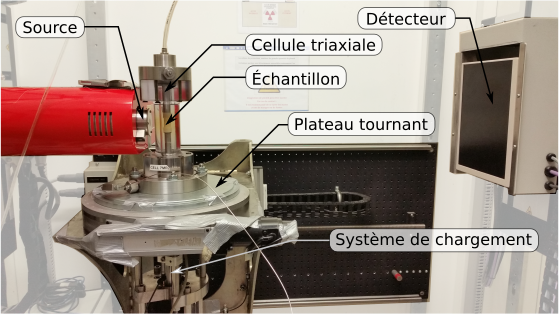
\includegraphics[]{tomo/manip.png}
			\caption{\label{fig04:manip_tomo}Photographie annotée du dispositif de tomographie du laboratoire 3SR utilisé dans ces travaux. Le fond a été mis en transparence pour des raisons de clarté.}
		\end{figure}
		Les paramètres d'acquisition des images de tomographie, pour les essais de compression triaxiale menés dans le tomographe, sont présentés dans le tableau \ref{tab04:param_tomo}. Le voltage et l'ampérage sont définis de manière à obtenir une puissance de faisceau des rayons X acceptables. Le faisceau doit être assez puissant pour traverser l'ensemble du dispositif expérimental et permettre un contraste entre les grains, l'air et la membrane. Il ne doit cependant pas être trop puissant pour ne pas saturer le détecteur.
		\\Le nombre de projection correspond au nombre de pas que le plateau tournant accomplit pour faire un tour complet. Pour chaque pas, le plateau reste fixe le temps de prendre au moins une radiographie de l'échantillon, que l'on nomme par la suite projection. Le nombre d'images par projection correspond au nombre de radiographies prises pour créer une projection. Plus le nombre de radiographies est grand, plus le bruit de l'image est diminué puisque le signal moyen de l'ensemble des radiographies prises est considéré pour établir la projection. De même, plus le nombre de projections augmente, plus la netteté de l'image reconstruite est élevée puisque le processus de reconstruction utilise plus de données brutes.
		\begin{table}\centering
			\begin{tabular}{rccc}
				\cline{2-4}
				& Confinement & Confinement & Confinement\\
				& \SI{1}{\mega\pascal} & \SI{2}{\mega\pascal} & \SI{7}{\mega\pascal}\\\hline
				Taille du voxel [\si{\micro\meter}] & 9.00 & 9.00 & 9.00 \\\hline
				Voltage [\si{\kilo\volt}] & 80 & 80 & 80 \\\hline
				Ampérage [\si{\micro\ampere}] & 112 & 113 & 125 \\\hline
				Nombre de projections & 1440 & 1440 & 1120 \\\hline
				Images par projection & 3 & 3 & 6 \\\hline
				\multirow{2}{*}{Volume [\si{\voxel^3}]} & $1445\times 1445$ & $1445\times 1445$ & $1444\times 1444$ \\
				& $\times 1600$ & $\times 1600$ & $\times 1650$ \\\hline
			\end{tabular}
			\caption{\label{tab04:param_tomo}Paramètres d'acquisition des images de tomographie pour les différents essais réalisés \textit{in situ}.}
		\end{table}
	\subsection{Utilisation des projections et reconstruction}
		La reconstruction des images de tomographie à partir des projections est expliquée au paragraphe \ref{para03:tomo}. Seulement, l'étape de reconstruction ne consiste pas uniquement à la superposition des différentes projections. Il est nécessaire de corriger certains artefacts liés à l'acquisition des images dans le même temps. Cela a été réalisé par l'intermédiaire du programme XAct.
		\\Un scan est caractérisé par l'acquisition de l'ensemble des projections, et donc à la prise de radiographies sous une multitude d'angles d'acquisition de $0$ à $360$ degrés. Comme pour toute prise d'images, il est primordial que le sujet ne bouge pas en cours d'acquisition afin d'assurer une netteté correcte de l'image. Compte tenu des performances du tomographe du laboratoire utilisé, du nombre de projections par scan et du nombre d'images par projection, le temps de scan est plutôt conséquent : il faut compter en moyenne deux heures. Durant ces deux heures, il est possible que la microstructure de l'échantillon ait été modifiée ou que l'échantillon se soit déplacé. La microstructure étant stable lors des phases de scan, seul le déplacement de l'échantillon en cours d'acquisition des projections est observé. Afin de tenir compte de ce déplacement en cours d'acquisition, trente-deux projections sont réalisées sur des angles linéairement répartis entre $0$ et $360$ degrés et sur des positions déjà traitées. Un calcul de corrélation entre les projections "normales" et les projections en fin de scan permet d'établir le déplacement de l'échantillon en cours d'acquisition et de corriger la position de la microstructure lors de la reconstruction.
		\begin{figure}\centering
			\subfloat[Exemple de projection radiographique]{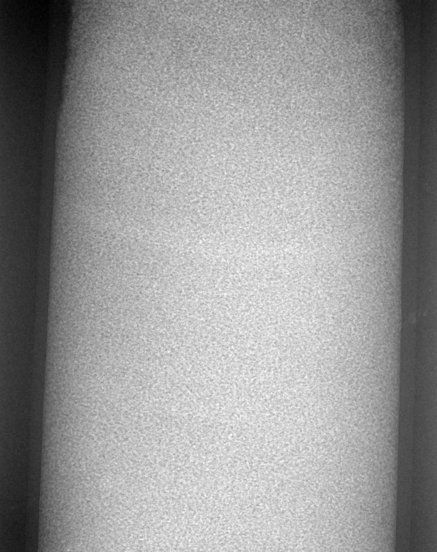
\includegraphics[width=.6\textwidth]{tomo/proj_rescale_15.jpg}}\\
			\subfloat[Coupe horizontale après reconstruction]{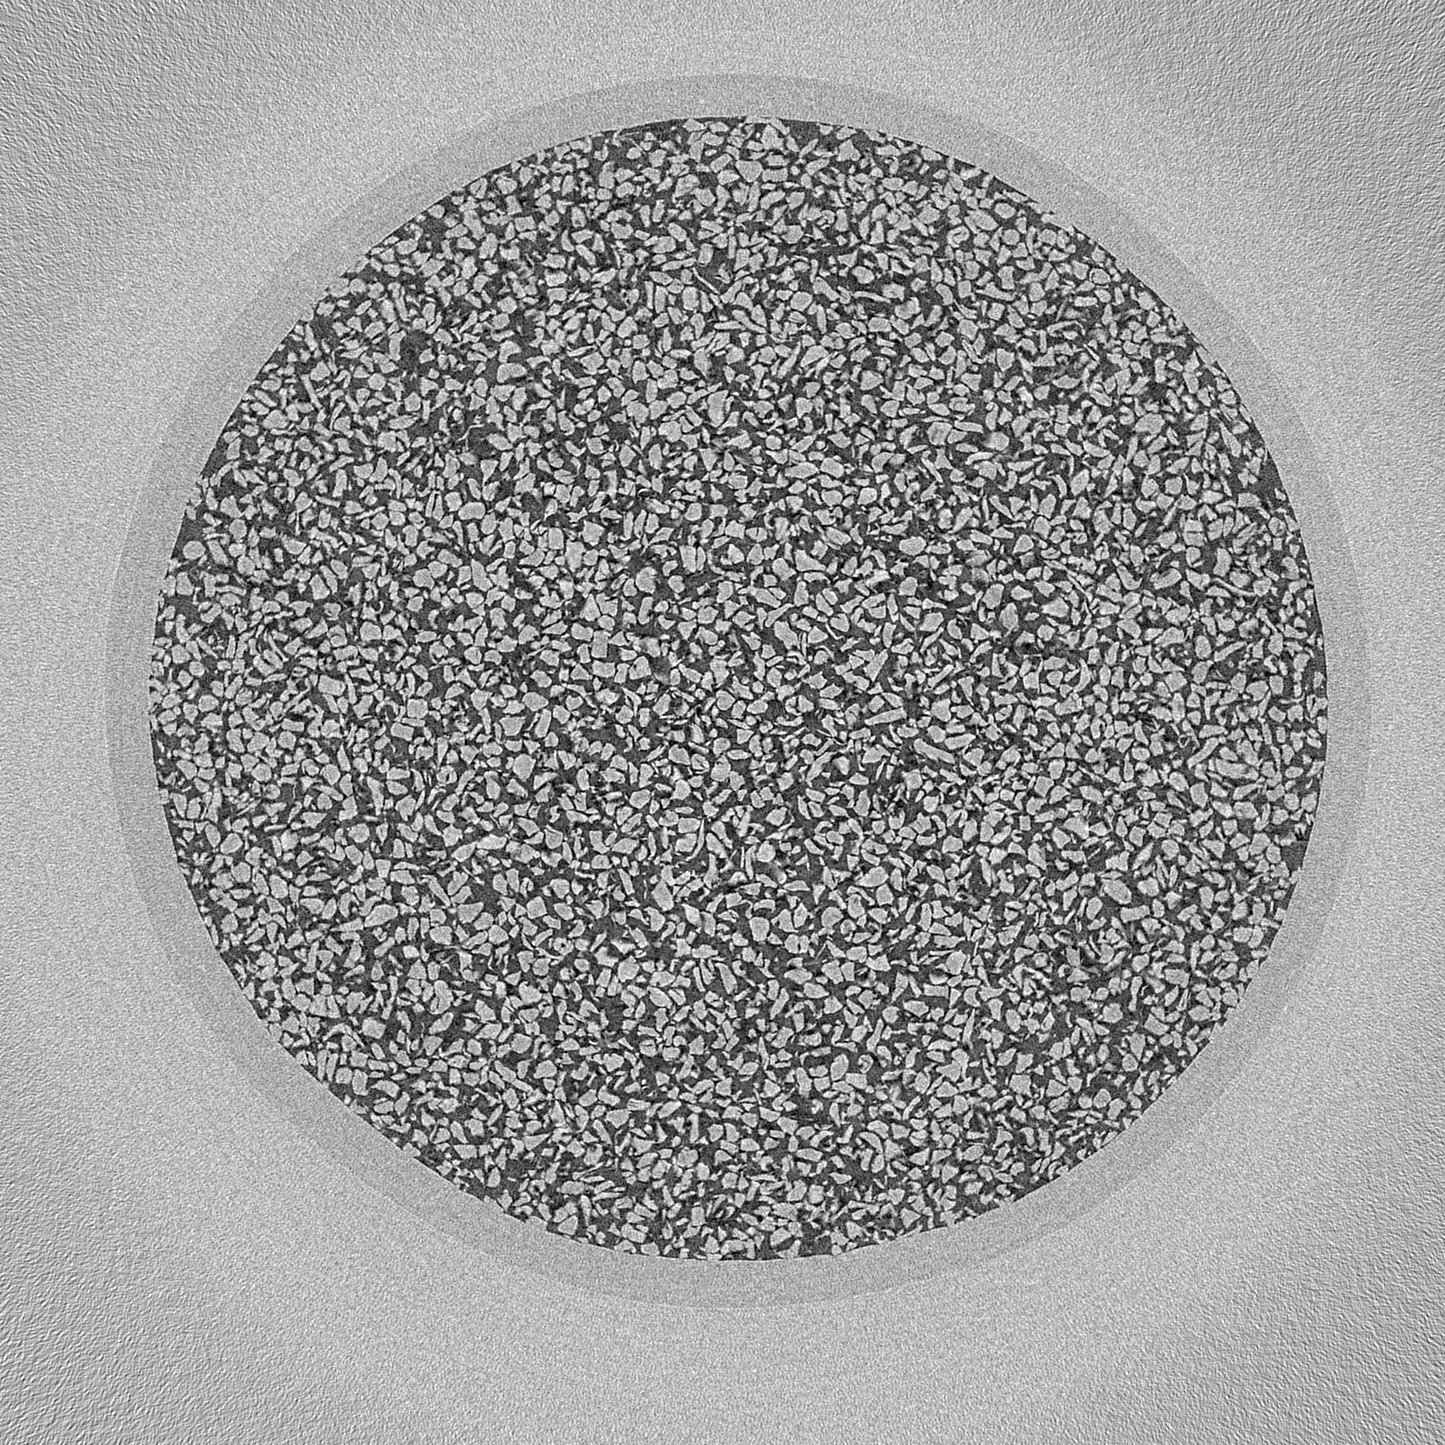
\includegraphics[width=.55\textwidth]{tomo/slice.jpg}}\hfill
			\subfloat[Volume 3D après reconstruction]{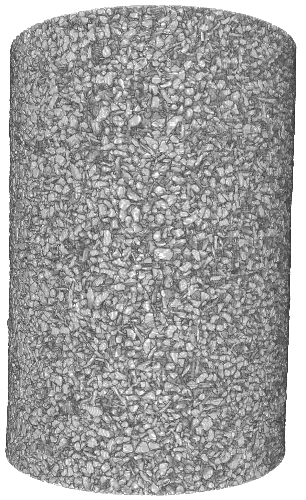
\includegraphics[width=.35\textwidth]{tomo/3D_0_00.jpg}}
			\caption{\label{fig04:reconstruction_tomo}Les projections (a) issues de la tomographie permettent d'obtenir, par reconstruction, des coupes internes de l'échantillon (b) et la microstructure du volume complet (c).}
		\end{figure}
		\begin{figure}\centering
			\subfloat[\SI{1}{\mega\pascal} - $E_0$]{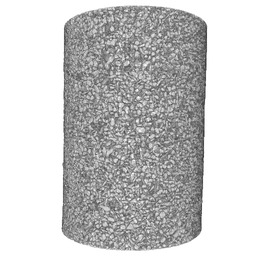
\includegraphics[width=0.33\textwidth]{3d_samples/1_00_resized.jpg}}\hfill
			\subfloat[\SI{1}{\mega\pascal} - $E_C$]{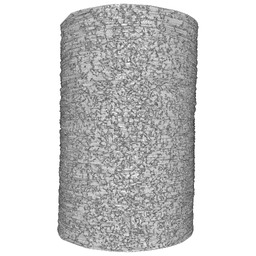
\includegraphics[width=0.33\textwidth]{3d_samples/1_0Pc_resized.jpg}}\hfill
			\subfloat[\SI{1}{\mega\pascal} - $E_F$]{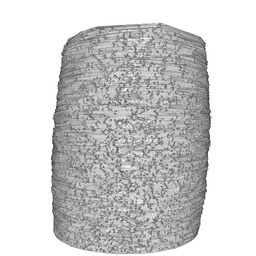
\includegraphics[width=0.33\textwidth]{3d_samples/1_8_resized.jpg}}
			\\
			\subfloat[\SI{2}{\mega\pascal} - $E_0$]{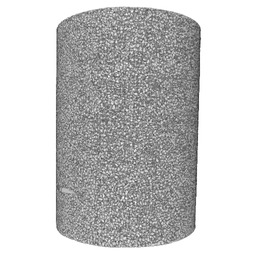
\includegraphics[width=0.33\textwidth]{3d_samples/2_00_resized.jpg}}\hfill
			\subfloat[\SI{2}{\mega\pascal} - $E_C$]{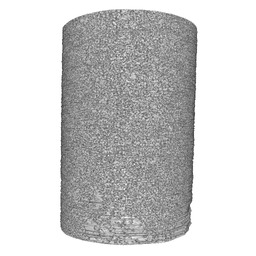
\includegraphics[width=0.33\textwidth]{3d_samples/2_0Pc_resized.jpg}}\hfill
			\subfloat[\SI{2}{\mega\pascal} - $E_F$]{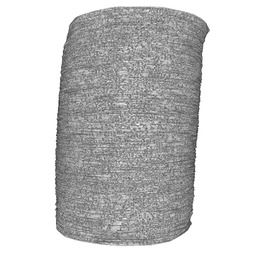
\includegraphics[width=0.33\textwidth]{3d_samples/2_9_resized.jpg}}
			\\
			\subfloat[\SI{7}{\mega\pascal} - $E_0$]{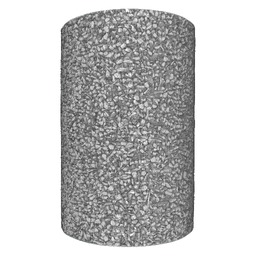
\includegraphics[width=0.33\textwidth]{3d_samples/7_00_resized.jpg}}\hfill
			\subfloat[\SI{7}{\mega\pascal} - $E_C$]{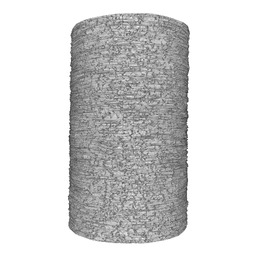
\includegraphics[width=0.33\textwidth]{3d_samples/7_0Pc_resized.jpg}}\hfill
			\subfloat[\SI{7}{\mega\pascal} - $E_F$]{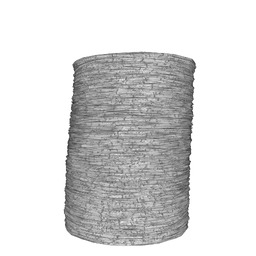
\includegraphics[width=0.33\textwidth]{3d_samples/7_7_resized.jpg}}
			\caption{\label{fig04:samples_3D}Représentation des reconstructions volumiques de chacun des échantillons (\SI{1}{\mega\pascal}, \SI{2}{\mega\pascal} et \SI{7}{\mega\pascal} en fonction de la pression de confinement) dans différents états de compression : $E_0$ est l'état non comprimé (dit naturel), $E_C$ est l'état de compression isotrope (après la mise en confinement) et $E_F$ est l'état final (après le dernier chargement axial).}
		\end{figure}
		\\\`A la suite de la correction liée au déplacement de l'échantillon, la superposition des projections peut être faite. Avant cela, un échantillonnage du signal est réalisé pour former des reconstructions au format 16-bit. Pour cela, des valeurs limites lues par le détecteur des rayons X sont choisies. Toutes les valeurs inférieures à la plus petite valeur limite sont considérées égales à 0, celles supérieures à la plus grande valeur limite sont considérées égales à \num{65535} ($2^{16}-1$). Les valeurs intermédiaires suivent la même répartition linéaire que celle du signal d'origine entre les deux valeurs limites.
		La figure \ref{fig04:reconstruction_tomo} (a) présente un exemple de projection obtenu lors d'un scan dans le tomographe. L'ensemble des corrections appliquées aux projections et la superposition des projections permettent d'obtenir la microstructure du volume scanné. Les figures \ref{fig04:reconstruction_tomo} (b) et (c) en sont des exemples. La première représente une coupe dans le volume suivant à une hauteur donnée de l'échantillon tandis que la seconde représente le volume. La figure \ref{fig04:samples_3D} présente quant à elle les volumes des échantillons avant la mise en confinement, après la mise en confinement et après le chargement axial final pour chacun des trois essais.

\section{Caractérisation des échantillons}
	Les images de tomographie acquises durant les essais de compression triaxiale vont permettre d'analyser la microstructure des échantillons puisqu'elles caractérisent directement l'état de densité de ces derniers. Cependant l'utilisation immédiate de ces images n'est pas recommandée et un traitement du signal de chacune d'elles est nécessaire pour optimiser les méthodes d'analyse. Ces méthodes consistent à cartographier les états de densité et de déformation (en menant des calculs de corrélation de volumes numériques) au sein de l'échantillon afin de permettre une étude locale, mais également globale, des échantillons en cours de compression.
	\subsection{Post-traitement des images de tomographie}
		\subsubsection{Traitement et optimisation des images}
			Les images directement issues des reconstructions de tomographie ne sont pas adaptées pour être analysées. En effet, en fonction du protocole suivi pour la tomographie et des limites du tomographe, les images peuvent se retrouver mal contrastées et bruitées. Il est alors nécessaire de corriger la qualité de ces images par des méthodes simples et bien connues. Les reconstructions de tomographie sont des images au format 8-bit. L'ensemble des tâches présentées ici sont adaptées à ce format d'image. La plage d'intensité des voxels pour ce format est l'ensemble des entiers positifs allant de $0$ à $255$ compris.
			\\La tomographie ayant été réalisée sur un échantillon comprimé d'une poudre constituée d'un seul matériau, nous nous attendons à observer un signal bimodal. En effet, le milieu observé est constitué de deux éléments : le polystyrène qui absorbe assez bien les rayons X et l'air comblant les porosités qui absorbe très peu ces mêmes rayons. Puisque la tomographie est basée sur une technique d'absorption des rayons X (cf. paragraphe \ref{para03:tomo}), il est logique d'observer une grande partie des voxels ayant une intensité relativement grande et une une autre grande partie relativement faible.
			\\Dans le cas idéal, avec des instruments de très grande résolution, des capteurs très performants et un milieu observé assurément isolé des conditions extérieures et complètement biphasique, l'histogramme des images reconstruites par tomographie devrait présenter deux pics uniques et totalisant l'ensemble des voxels (cf. paragraphe \ref{para03:traitement_image}). Parce que ces conditions ne sont pas réunies, on observe un signal plus lissé et plus bruité. L'histogramme présente alors deux pics plus ou moins étalés sur l'ensemble des valeurs d'intensité des voxels. Afin d'analyser et d'utiliser les images de la manière la plus pertinente possible, il est nécessaire de se rapprocher du cadre idéal pour un milieu biphasique. Il est alors nécessaire de minimiser la largeur des pics de l'histogramme et de les éloigner le plus possible l'un de l'autre en augmentant le contraste. La figure \ref{fig04:contrast_enhancement_filtering} illustre l'ensemble des tâches accomplies afin de permettre cela. Chacune de ces étapes est décrite dans les paragraphes qui suivent.
			\begin{figure}\centering
				\subfloat[Image d'origine]{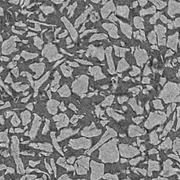
\includegraphics[width=.27\textwidth]{contrast_enhancement_filtering/00-orig_0142_resized.png}}
				\subfloat[Histogramme de l'image d'origine]{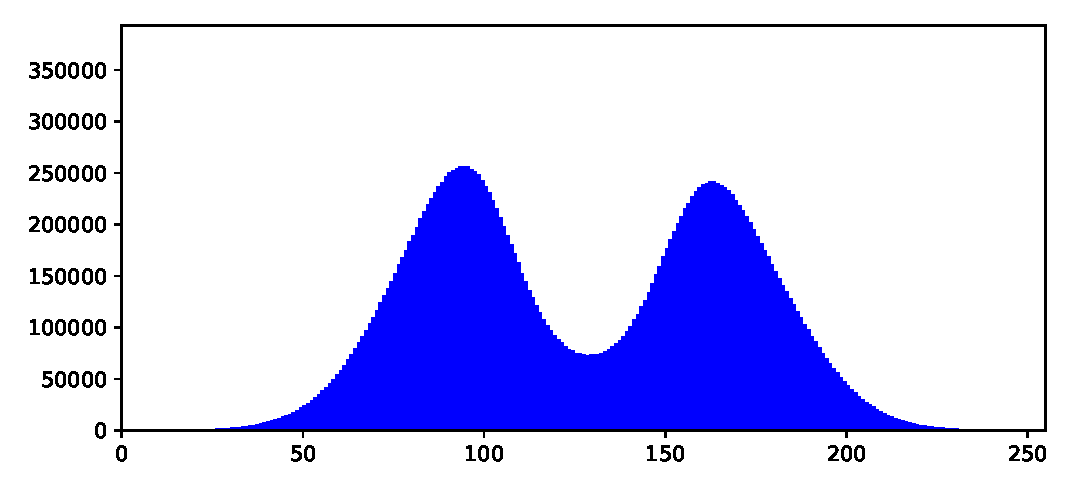
\includegraphics[width=.67\textwidth]{contrast_enhancement_filtering/00-orig_hist.eps}}\\
				\subfloat[Accentuation du contraste]{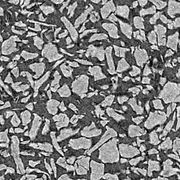
\includegraphics[width=.27\textwidth]{contrast_enhancement_filtering/01-contrast_0142_resized.png}}
				\subfloat[Histogramme de l'image avec accentuation du contraste]{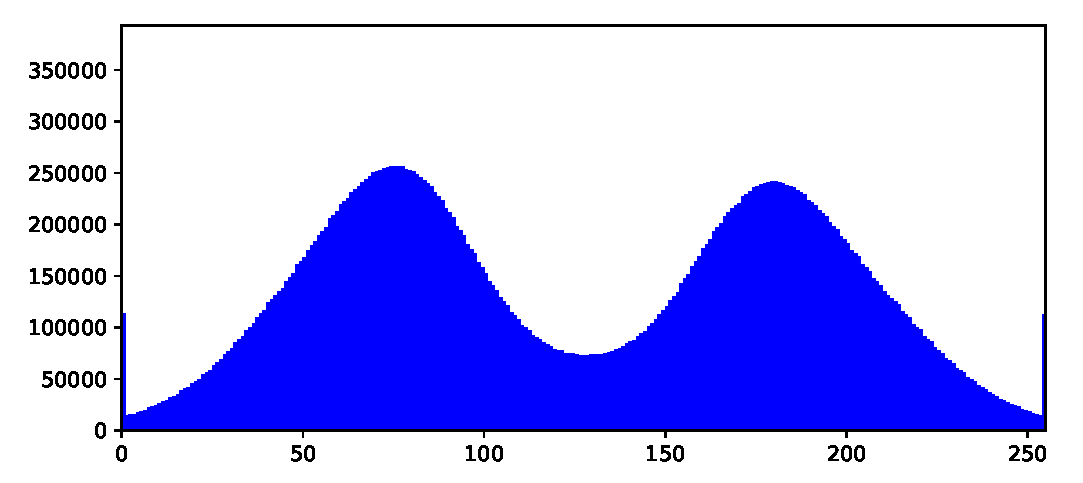
\includegraphics[width=.67\textwidth]{contrast_enhancement_filtering/01-contrast_hist.eps}}\\
				\subfloat[Filtre bilatéral]{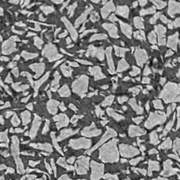
\includegraphics[width=.27\textwidth]{contrast_enhancement_filtering/02-bilat_0142_resized.png}}
				\subfloat[Histogramme de l'image avec filtre bilatéral]{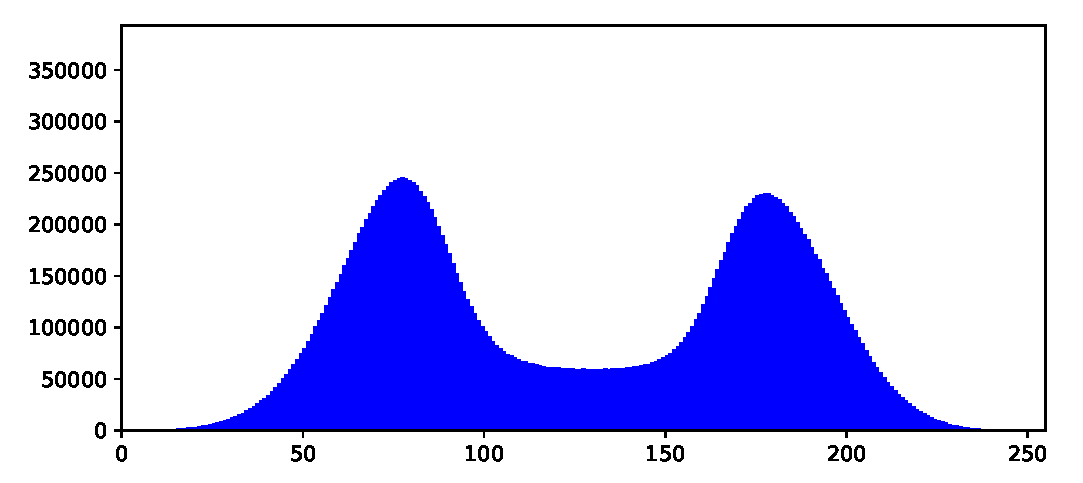
\includegraphics[width=.67\textwidth]{contrast_enhancement_filtering/02-bilat_hist.eps}}\\
				\subfloat[Filtre de variation totale]{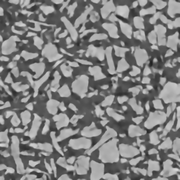
\includegraphics[width=.27\textwidth]{contrast_enhancement_filtering/03-bilatTV_0142_resized.png}}
				\subfloat[Histogramme de l'image avec filtre de variation totale]{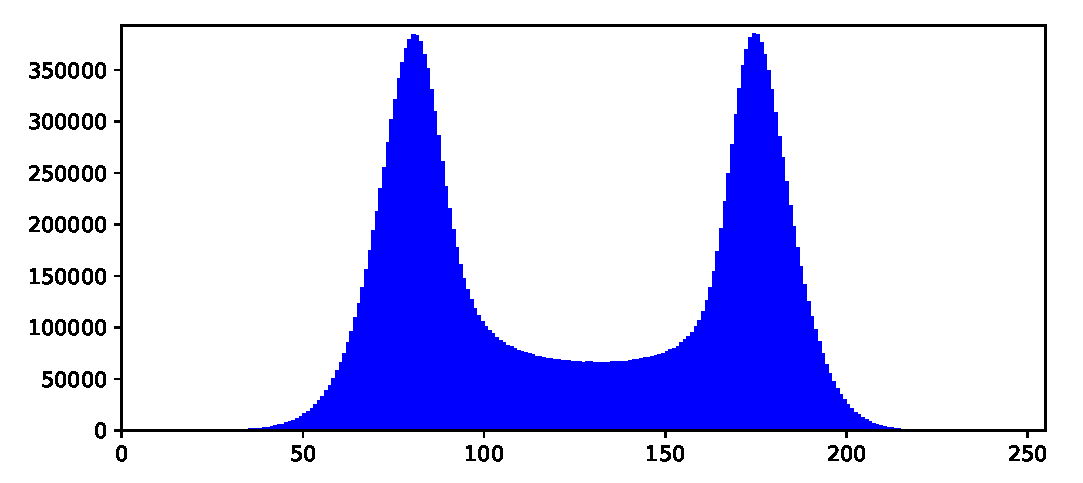
\includegraphics[width=.67\textwidth]{contrast_enhancement_filtering/03-bilatTV_hist.eps}}
				\caption{\label{fig04:contrast_enhancement_filtering}Illustration du traitement des images issues des reconstructions de tomographie. A gauche, une coupe de l'image 3D. A droite, l'histogramme associé à cette image 3D.}
			\end{figure}
			\paragraph{}La première étape consiste à atténuer le bruit aux extrémités de la plage de données du signal et procéder à un renforcement du contraste. Cette étape est illustrée sur les figures \ref{fig04:contrast_enhancement_filtering}-(c) et (d). Il est considéré que le bruit est présent sur l'ensemble de la plage de données du signal (pour toutes les nuances de gris) alors que l'information structurale de l'échantillon n'est présente que sur une zone plus restreinte et centrée sur cette même plage de données. Pour les travaux de cette thèse, il a été considéré que l'information structurale est donnée dans les \num{99} percentiles centrés sur la plage de données (qui va de \num{0} à \num{255}). Considérant cela, les voxels ayant une intensité plus faible que l'intensité du voxel à \num{0.5} percentile ($I_\textrm{min}$) prennent la valeur de ce dernier. Les voxels ayant une intensité plus grande que le voxel à \num{99.5} percentile ($I_\textrm{max}$) prennent la valeur de ce dernier. Comme la nouvelle plage d'intensités prises par les voxels est désormais plus petite que celle d'origine ($I_\textrm{max}-I_\textrm{min} < 255$), il est nécessaire d'étaler de manière uniforme le nouveau signal entre les valeurs $0$ et $255$. L'équation (\ref{eq04:contraste}) permet de déterminer la valeur de l'intensité d'un voxel après renforcement du contraste ($I_\textrm{après}$) en fonction de l'intensité du même voxel dans l'image d'origine ($I_\textrm{avant}$).
			\begin{equation}\label{eq04:contraste}
			I_\textrm{après} = \cfrac{I_\textrm{avant} - I_\textrm{min}}{I_\textrm{max} - I_\textrm{min}}\times 255
			\end{equation}
			\paragraph{}La seconde étape, illustrée sur les figures \ref{fig04:contrast_enhancement_filtering}-(e), (f), (g) et (h), consiste à lisser le signal de manière à éliminer le bruit au sein de chaque phase. Cela se fait par l'intermédiaire de filtres qui engendrent un flou dans l'image. Cette étape permet de mieux identifier les pics présents dans l'histogramme mais peut avoir pour conséquence de rendre la limite entre ces deux pics plus difficile à établir. Les voxels qui sont proches des frontières entre les deux phases vont également subir le flou et vont prendre des valeurs intermédiaires. Sur l'histogramme, les deux pics seront donc mieux définis car plus fins mais le minimum situé entre ces deux pics sera augmenté à cause des voxels aux frontières. Un moyen d'éviter ce dernier effet est d'engendrer un flou qui tient compte des bordures et donc des zones à fort contraste. Pour cette raison, les filtres de lissage "bilatéral" \citep{tomasi_bilateral_1998} et "variation totale" \citep{chambolle_algorithm_2004} ont été choisis. Le filtre bilatéral modifie la valeur des voxels en moyennant la valeur des voxels voisins qui n'ont pas tous le même poids dans la moyenne. Le poids attribué à chaque voxel voisin dépend de la distance euclidienne avec le voxel en cours de traitement (plus il est proche et plus il compte dans la moyenne - il s'agit de la même approche que pour un lissage gaussien) mais également de la différence de niveau de gris entre les deux voxels (plus la différence est grande, moins il compte dans la moyenne - c'est cette propriété qui permet de conserver les frontières entre les différentes phases). Le filtre de variation totale est quant à lui basé sur la recherche d'une image qui minimise la variation totale du signal tout en restant le plus proche possible de l'image de départ ; il s'agit là encore d'un processus qui conserve plutôt bien les frontières entre différentes phases. Le choix a été fait d'utiliser successivement ces deux filtres afin de minimiser le temps et le coût de calcul. En effet, le filtre bilatéral semble être le plus efficace et suffit à lui seul à corriger les images. Cependant, l'ensemble des calculs non-linéaires qu'il doit fournir rend la tâche non adaptée au projet. Il est possible de l'utiliser sans engendrer trop d'énergie de calcul avec des paramètres permettant une correction relativement moyenne. Le filtre de variation totale permet de finaliser le lissage plus rapidement grâce aux calculs qui sont, cette fois-ci, linéaires.
			\paragraph{}La figure \ref{fig04:contrast_enhancement_filtering} montre l'effet de chacune des corrections sur une coupe de l'image 3D et son histogramme. Il est à noter que cette figure illustre les effets des corrections sur une image plane bien que ces corrections soient dans les trois directions de l'espace. Il est en effet difficile de visualiser des images 3D sur un support plan. Pour cette raison, des coupes seront exposées dans les plans les plus faciles à extraire : ce seront ici des coupes dans le plan ($Oxy$) d'un repère cartésien pour les reconstructions de tomographie. En effet, les images reconstruites ont été enregistrées sous la forme de "stack" qui correspond à un empilement d'image dans la direction de l'axe ($Oz$). Le filtre bilatéral est celui de la bibliothèque Python "scikit-image" \citep{scikit_image} et a pour paramètres : un écart-type spatial de \SI{2}{\voxel}, un écart-type d'intensité de \num{0.007} et une fenêtre de travail de \SI{6}{\voxel} de côtés. Le filtre de variation totale, issu de la même bibliothèque Python, a pour paramètre un poids de $0.1$. Ces valeurs ont été choisies de manière purement qualitative. Une comparaison des histogrammes de l'image d'origine (figure \ref{fig04:contrast_enhancement_filtering}-(b)) et de l'image traitée (figure \ref{fig04:contrast_enhancement_filtering}-(h)) permet d'identifier une augmentation de la grandeur des pics et une diminution de leur largeur. Ces éléments prouvent que le processus employé transforme l'image d'origine en une image plus facile à binariser, facilitant ainsi la reconnaissance des deux phases en présence.
		\subsubsection{Binarisation par seuillage automatique}
			\label{para04:seuillage}
			\paragraph{}La figure \ref{fig04:contrast_enhancement_filtering}-(h) met en évidence qu'une relativement grande partie des voxels ont des intensités comprises entre les deux valeurs caractérisant les pics, formant ainsi un plateau entre ceux-ci. La distinction entre les deux phases nécessite de déterminer une valeur limite sur ce plateau. La détermination de cette valeur limite, appelée valeur seuil, peut être réalisée en utilisant une méthode de seuillage automatique (cf. paragraphe \ref{para03:threshold}). Deux méthodes couramment utilisées sont décrites ici.
			\paragraph{}La première méthode de seuillage automatique est celle de \citet{otsu_threshold_1979}. Otsu montre que dans le cadre d'un signal bimodal, donc avec deux classes, une valeur seuil optimale est celle qui minimise la variance intra-classe\footnote{La variance intra-classe correspond à la moyenne des variances de chacune des classes.} du signal. Cela revient à maximiser la variance inter-classe\footnote{La variance inter-classe correspond à la variance des moyennes de chacune des classes.}. D'un point de vue pratique, la méthode de seuillage d'Otsu consiste à seuiller l'image pour toutes les valeurs possible de seuillage (de \num{0} à \num{255} pour une image au format 8-bit), de calculer les valeurs moyennes de chacune des phases et de mesurer la variance des moyennes obtenues. Une fois que cela est fait pour chacune des valeurs seuil possible, c'est la valeur seuil pour laquelle la variance est la plus grande qui va être choisie comme valeur seuil qui permet d'identifier les différentes phases.
			\paragraph{}La seconde méthode de seuillage a été développée par \citet{kittler_minimum_1986} et est souvent dénommée "méthode de seuillage par minimisation de l'erreur". Avec cette méthode, chacun des deux modes est approximé par une gaussienne. La valeur de seuil optimale est choisie lorsque le chevauchement entre les gaussiennes est minimal.
			\paragraph{}Les deux méthodes décrites ici ont chacune leurs avantages et sont toutes deux adaptées à la segmentation des images présentant deux phases (signal bimodal). Malgré cela, les méthodes de calcul de la valeur seuil étant différentes, les deux méthodes de seuillages n'indiquent pas les mêmes seuils. \'Evidemment, ces valeurs restent proches l'une de l'autre mais la différence est suffisante pour engendrer des erreurs d'analyse des images binaires par la suite. Il est difficile de définir la méthode la mieux adaptée puisque cela dépend directement du signal des images et de leur qualité. Dans certains cas la méthode d'Otsu sera plus adaptée que celle de Kittler et Illingworth, dans d'autres cas ce sera l'inverse. Il a été remarqué cependant que pour un milieu confiné donné (même milieu granulaire, même densité), avec des images issues d'un même protocole expérimental (même tomographe, même méthode de reconstruction, etc.), la qualité du seuillage reste la même pour différentes images. Il semble donc que la méthode à choisir dépende du milieu granulaire observé, de sa densité apparente et du protocole suivi pour la réalisation de la tomographie. Il est, par conséquent, nécessaire de définir une méthode de seuillage pour chaque échantillon observé par tomographie et pour chaque état de compression.
			\paragraph{}Il reste à résoudre un problème. Comment choisir parmi les deux méthodes de seuillage automatique ? Comment faire lorsque les deux méthodes ne donnent pas un résultats approprié ? On considère d'abord que les voxels les plus clairs (valeurs proches de \num{255}) sont ceux qui caractérisent le matériau constituant le milieu granulaire et ceux qui sont sombres (valeurs proches de \num{0}) caractérisent les porosités. Les images de tomographie utilisées dans ces travaux présentent toujours le même constat : le seuillage par la méthode d'Otsu présente une valeur seuil légèrement différente de celle de Kittler, de sorte que lorsque l'une semble trop basse l'autre semble trop élevée. Ainsi, en seuillant l'image par une méthode quelques voxels de porosité sont considérés comme de la matière tandis qu'avec la seconde méthode c'est l'inverse.
			\paragraph{}Une manière de régler le problème de choix entre les deux méthodes de seuillage est d'utiliser une moyenne pondérée. En faisant cela, un seul paramètre suffit pour déterminer la valeur seuil. Cette moyenne est calculée suivant l'équation (\ref{eq04:seuillage}) :
			\begin{equation}\label{eq04:seuillage}
			S = \alpha\cdot S_\textrm{Otsu} + \left(1-\alpha\right)\cdot S_\textrm{Kittler}
			\end{equation}
			avec, $S$ la valeur de seuil choisie entre la valeur seuil d'Otsu $S_\textrm{Otsu}$ et celle de Kittler $S_\textrm{Kittler}$, et $\alpha$ le paramètre de pondération qui représente le poids de la méthode d'Otsu sur cette moyenne. Comme il l'a été dit, la valeur de seuil ne semble pas varier pour un même milieu confiné. Il suffit donc de déterminer la valeur du coefficient $\alpha$ pour chaque essai de compression accompli au sein du tomographe, et pour chaque état de compression. C'est ce qui a été fait. Des tests ont été menés sur des images issues des différentes campagnes d'essais afin de déterminer les valeurs de $\alpha$. L'évaluation de la valeur de seuillage optimale a été entièrement qualitative, par méthode de visualisation et comparaison des images originales et binaires. Un réajustement de la valeur de $\alpha$ est nécessaire lors de toute analyse d'images nouvelles (issues d'un nouvel essai).
			\begin{table}\centering
				\begin{tabular}{ccc}
					\hline
					& \multicolumn{2}{c}{Milieu granulaire avec}\\
					& grains de polystyrène & grains d'amidon \\\hline
					Valeur du coefficient $\alpha$ & $0.2$ & $0.4$ \\\hline
				\end{tabular}
				\caption{\label{tab04:valeur_alpha}Valeurs du coefficient de pondération de la méthode d'Otsu concernant la moyenne pondérée avec la méthode de Kittler.}
			\end{table}
			Le tableau \ref{tab04:valeur_alpha} mentionne les valeurs moyennes utilisées pour calculer la valeur de seuillage la plus appropriée au milieu observé. On remarque que la méthode de Kittler semble, sur les échantillons étudiés dans cette thèse, plus pertinente que la méthode d'Otsu ($\alpha < 0.5$) et que la morphologie des grains et la granulométrie semblent jouer un rôle dans le choix de ce coefficient et donc de la valeur seuil.
			\begin{figure}\centering
				\subfloat[$\alpha = 1.0\quad\left( S=120 \right)$]{
					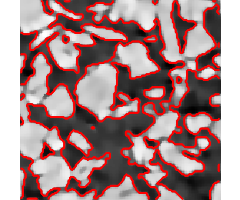
\includegraphics[width=0.3\textwidth]{threshold/contour_120_0142.png}}\hfill
				\subfloat[$\alpha = 0.4\quad\left( S=126 \right)$]{
					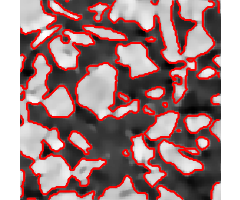
\includegraphics[width=0.3\textwidth]{threshold/contour_126_0142.png}}\hfill
				\subfloat[$\alpha = 0.0\quad\left( S=130 \right)$]{
					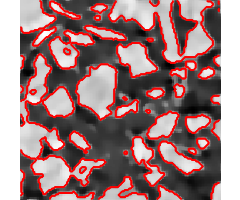
\includegraphics[width=0.3\textwidth]{threshold/contour_130_0142.png}}
				\\
				\subfloat[Visualisation sur l'histogramme de l'image 3D associée]{
					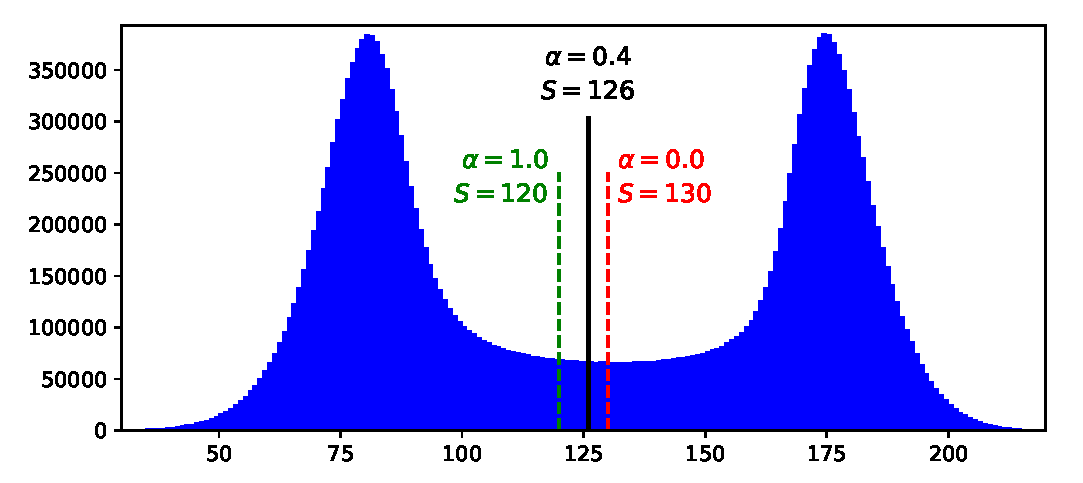
\includegraphics[width=0.8\textwidth]{threshold/histogram.eps}
				}
				\caption{\label{fig04:seuillage_polystyrene}Résultat du seuillage automatique avec différentes valeurs de $\alpha$. $S$ désigne la valeur de seuillage obtenue. Les figures (a), (b) et (c) représente une coupe de l'image 3D sur laquelle est superposée le contour des zones seuillées (en rouge).}
%				$\begin{array}{c}\alpha = 0.4\\S_{\alpha{_1}} = 120\end{array}$
			\end{figure}
			\\Les figures \ref{fig04:seuillage_polystyrene}-(a) à (c) illustrent l'effet du paramètre $\alpha$ sur une coupe d'image de tomographie d'un milieu constitué de grains de polystyrène. La méthode d'Otsu (figure \ref{fig04:seuillage_polystyrene}-(a)) a tendance à diminuer la porosité. C'est l'inverse avec la méthode de Kittler (figure \ref{fig04:seuillage_polystyrene}-(c)). La moyenne pondérée des deux méthodes avec $\alpha=0.4$ permet de considérer le seuillage optimal. La figure \ref{fig04:seuillage_polystyrene}-(d) permet d'observer l'effet du seuillage directement sur l'histogramme.
	\subsection{Analyse de densité}
		L'image seuillée obtenue par binarisation est une image représentant les deux phases de l'échantillon : les voxels blancs représentent les grains tandis que les voxels noirs représentent les porosité à l'intérieur du milieu granulaire. \`A partir de cette information sur l'image binaire, il est possible de mesurer la densité\footnote{Il s'agit en fait de calculer la fraction volumique solide qui peut être considérée comme identique à la densité dans le cas d'un milieu constitué d'un seul matériau incompressible.} $d$ du milieu dans un volume donné $V$, constitué de $V_G$ voxels blancs et $V_P$ voxels noirs, grâce à l'équation (\ref{eq04:calcul_densite}) :
		\begin{equation}\label{eq04:calcul_densite}
			d = \cfrac{V_G}{V} = \cfrac{V_G}{V_G+V_P}
		\end{equation}
		Lorsque l'équation (\ref{eq04:calcul_densite}) est utilisée sur le volume entier de l'échantillon, la densité obtenue correspond alors à la densité apparente de l'échantillon $d_\textrm{ech}$ qui est calculée expérimentalement avec la masse de grain introduite $m$, la masse volumique du matériau constituant les grains $\rho$ et le volume de l'échantillon $V_\textrm{ech}$ par la relation (\ref{eq04:mesure_densite}) :
		\begin{equation}\label{eq04:mesure_densite}
			d_\textrm{ech} = \cfrac{m}{\rho V_\textrm{ech}}
		\end{equation}
		Cette dernière équation donne une information sur la densité de l'échantillon dans sa globalité. La figure \ref{fig04:bulkDensities} montre l'évolution de la densité relative globale des échantillons pour chacun des essais et calculée à partir de (\ref{eq04:calcul_densite}) sur l'ensemble des volumes issus des scans de tomographie. Le graphe représente l'évolution de cette densité en fonction de la déformations axiale imposée. Alors que la densité de l'échantillon subissant une pression de confinement de \SI{7}{\mega\pascal} est une contribution presque linéaire de la déformation axiale, il n'en est pas de même pour les pressions de confinement inférieures (\num{1} et \SI{2}{\mega\pascal}). Une explication possible à cela \citep{pavier_caracterisation_1998} est que l'élévation de la pression de confinement favorise la déformation des grains (qui sont ductiles) dans les zones de fortes contraintes de cisaillement en dépit du glissement pur (sans déformation). Ainsi, les échantillons des essais menés avec les plus faibles pressions de confinement seraient plus sensibles aux effets de dilatance et pourraient même présenter des bandes de cisaillement (cf. paragraphe \ref{para03:dilatance}). Ces raisons peuvent même expliquer la formation d'une géométrie "en tonneau" de l'échantillon pour les grandes déformations axiales (augmentation du volume apparent dans les zones de fort cisaillement). Il faut cependant rester vigilant sur ces résultats puisque, pour rappel, le calcul de densité est basée sur l'étude d'images binaires. Si la méthode de seuillage n'est pas adaptée pour l'un des états de chargement alors le calcul de densité s'en retrouve faussé. Or, bien que visuellement le seuillage des volumes les plus comprimés semble correct, la méthode de seuillage automatique utilisée dans ces travaux (cf. partie précédente) ne sera pas aussi efficace d'un état de compression à un autre.
		\begin{figure}\centering
			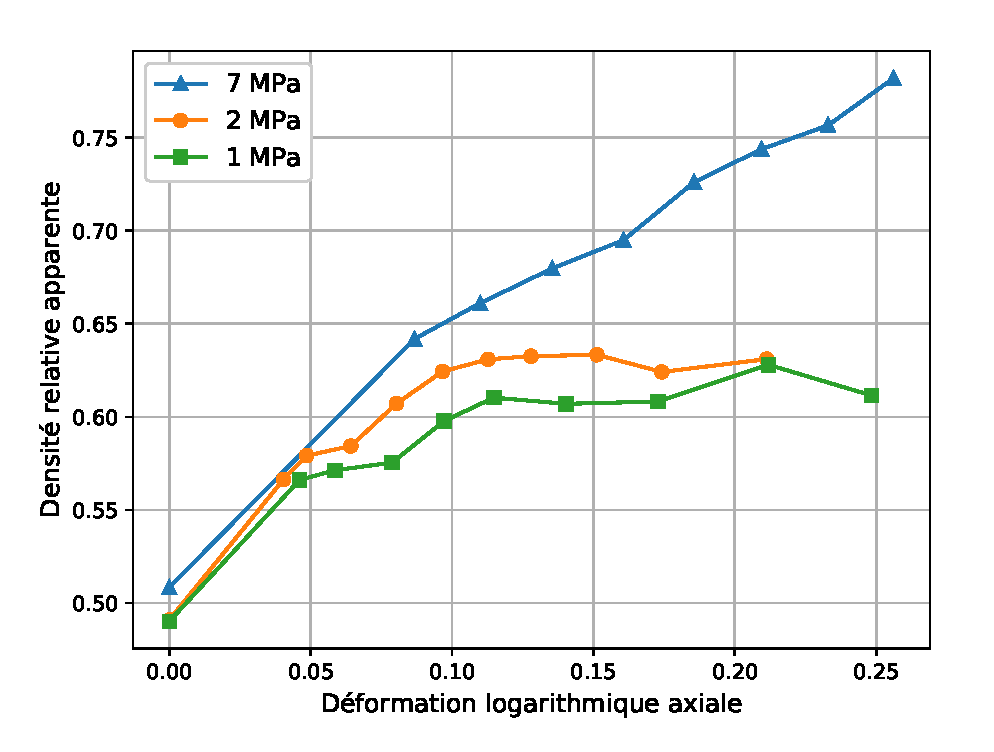
\includegraphics[width=0.8\textwidth]{bulkDensities/bulk_densities.eps}
			\caption{\label{fig04:bulkDensities}\'Evolution de la densité apparente des différents échantillons par rapport à la déformation axiale.}
		\end{figure}
		\paragraph{}
		Il peut être également intéressant d'étudier la densité de manière plus locale en utilisant l'équation (\ref{eq04:calcul_densite}) sur des volumes suffisamment petits pour suivre localement la densification de l'échantillon au cours de la compression. La discrétisation du volume total de l'échantillon $V_\textrm{ech}$ en sous-volumes $V_{\textrm{loc},i}$ selon les conditions données par (\ref{eq04:conditions_Vlocaux}) permet de générer un champ de densité dans l'échantillon.
		\begin{equation}\label{eq04:conditions_Vlocaux}
			\bigcup_i V_{\textrm{loc},i} = V_\textrm{ech}
			\qquad\text{et}\qquad
			\bigcap_i V_{\textrm{loc},i} = \emptyset
		\end{equation}
		Les images de tomographie obtenues dans ces travaux ont une dimension moyenne de $1450 \times 1450 \times 1600$ voxels et sont au format 8-bit : leur taille moyenne en mémoire est donc de $1450 \times 1450 \times 1600 / 2^{20} = 3208$ Mo ($2^{20}$ représente la valeur de $1$ Mo) soit encore \num{3.2} Go. Une discrétisation en sous-volumes cubiques de côté \SI{10}{\voxel} permet de travailler avec une image de dimension $145 \times 145 \times 160$ voxels et dont la taille en mémoire ne vaut plus que \num{3.2} Mo. En plus de cela, sachant que la taille des voxels dans les travaux menés dans cette thèse est de \SI{9}{\micro\meter}, les sous-volumes cubiques d'arête \SI{10}{\voxel} dans l'image numérique représentent finalement des sous-volumes dont les côtés ont une longueur de \SI{90}{\micro\meter} dans l'échantillon réel. Cette longueur est moins grande que celle de la taille moyenne des grains de polystyrène. Finalement, pour la définition donnée précédemment de sous-volumes, la "compression" du champ de densité donné directement par la tomographie permet d'obtenir un nouveau champ de densité dont la résolution permet encore d'informer localement de l'état de densification de l'échantillon à l'échelle du grain. Des cartes 3D des densités, comme celles présentées à titre d'exemple sur la figure \ref{fig04:densities_3D}, peuvent alors être calculées et permettre une analyse rapide et efficace de la densification des différents échantillons en cours de compression.
		\begin{figure}\centering
			\subfloat[\SI{1}{\mega\pascal} - $E_0$]{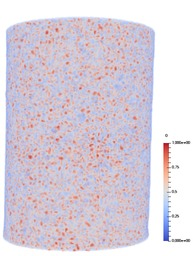
\includegraphics[width=0.27\textwidth]{3d_densities/1_00_resized.jpg}}\hfill
			\subfloat[\SI{1}{\mega\pascal} - $E_C$]{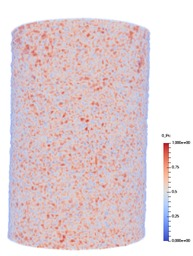
\includegraphics[width=0.27\textwidth]{3d_densities/1_0Pc_resized.jpg}}\hfill
			\subfloat[\SI{1}{\mega\pascal} - $E_F$]{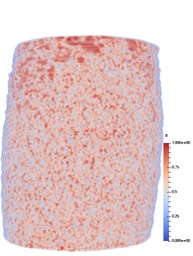
\includegraphics[width=0.27\textwidth]{3d_densities/1_8_resized.jpg}}
			\\
			\subfloat[\SI{2}{\mega\pascal} - $E_0$]{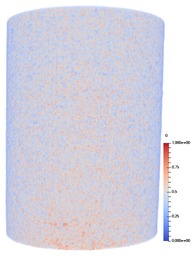
\includegraphics[width=0.27\textwidth]{3d_densities/2_00_resized.jpg}}\hfill
			\subfloat[\SI{2}{\mega\pascal} - $E_C$]{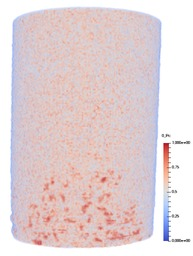
\includegraphics[width=0.27\textwidth]{3d_densities/2_0Pc_resized.jpg}}\hfill
			\subfloat[\SI{2}{\mega\pascal} - $E_F$]{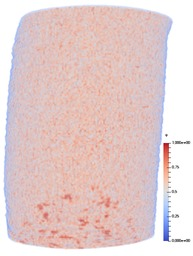
\includegraphics[width=0.27\textwidth]{3d_densities/2_9_resized.jpg}}
			\\
			\subfloat[\SI{7}{\mega\pascal} - $E_0$]{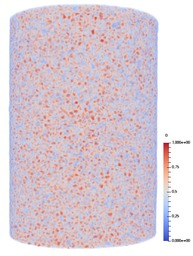
\includegraphics[width=0.27\textwidth]{3d_densities/7_00_resized.jpg}}\hfill
			\subfloat[\SI{7}{\mega\pascal} - $E_C$]{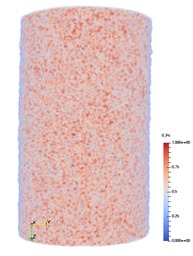
\includegraphics[width=0.27\textwidth]{3d_densities/7_0Pc_resized.jpg}}\hfill
			\subfloat[\SI{7}{\mega\pascal} - $E_F$]{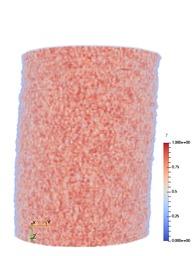
\includegraphics[width=0.27\textwidth]{3d_densities/7_7_resized.jpg}}
			\caption{\label{fig04:densities_3D}Représentation des champs de densité de chacun des échantillons dans différents états de compression en utilisant le même formalisme que pour la figure \ref{fig04:samples_3D}. La résolution de la mesure du champ est telle qu'un volume élémentaire de densité est un cube d'arrête de \SI{90}{\micro\meter}. L'échelle de couleur va du bleu pour une densité nulle jusqu'à du rouge pour une densité relative de $1$.}
		\end{figure}
	
	\subsection{Calcul de la cinématique}\label{para04:cinematique}
		En plus de l'évolution de la densité, il est possible de déterminer l'évolution des déformations dans l'échantillon en cours de compression. Cela est rendu possible par l'intermédiaire de la corrélation d'image 3D. Comme expliqué dans le paragraphe \ref{para03:DIC}, la corrélation des volumes issus de la tomographie permet d'obtenir un champ vectoriel des déplacements au sein des volumes. La cohérence des champs de déplacement obtenus a été vérifiée visuellement sur plusieurs sous-volumes choisis aléatoirement dans l'échantillon scanné. Les déplacements obtenus par l'intermédiaire du calcul de corrélation permettent en effet de suivre les mêmes grains tout au long du chargement mécanique. Il reste cependant difficile de qualifier l'erreur d'un point de vue quantitatif.
		\\A partir des champs de déplacement, on remonte aux champs des déformations par l'intermédiaire de l'opérateur gradient. Les grandes déformations ont été supposées et l'équation (\ref{eq04:defo_DVC}) est utilisée pour le calcul du tenseur des déformations de Green-Lagrange à partir du champ de déplacement.
		\begin{equation}\label{eq04:defo_DVC}
		\begin{array}{r@{\ =\ }l}
			\multicolumn{2}{l}{\forall i,j,k = 1,2,3}\\
			\varepsilon_{ij} & \cfrac{1}{2}\left( \left(\grad\ \underline{u}\right)_{i,j} + \left(\grad\ \underline{u}\right)_{j,i} + \left(\grad\ \underline{u}\right)_{k,i} \cdot \left(\grad\ \underline{u}\right)_{k,j}\right)\vspace{2mm}\\
			 & \cfrac{1}{2}\left( \partialdiff{u_i}{x_j} + \partialdiff{u_j}{x_i} + \partialdiff{u_k}{x_i} \partialdiff{u_k}{x_j} \right)
		\end{array}
		\end{equation}
		Le processus de calcul des champs de déformations est réalisé entre chaque étape de compression, lorsque deux scans ont été réalisés dans deux états successifs de compression. Le champ des déplacements obtenu par corrélation des volumes est défini en un certain nombre de n\oe{}uds : il s'agit du centre de chaque fenêtre de corrélation (imagette). Dans les travaux réalisés pour cette thèse, les fenêtres de corrélation sont de forme cubique avec des arêtes de \SI{10}{\voxel} sur le volume numérique, soit \SI{90}{\micro\meter} dans l'échantillon réel. Il s'agit finalement d'une grille 3D régulière qui indique le déplacement de sous-volumes cubiques, dont la taille est de \SI{90}{\micro\meter} soit la moitié d'un grain moyen, au sein de l'échantillon. Cette grille volumique régulière donne, pour chaque sous-volume, trois informations (les déplacements selon chacune des directions de l'espace). Le résultat de la corrélation des volumes peut donc être une combinaison de trois champs de déplacement distincts (un pour chaque direction de l'espace). La fonction \emph{gradient} du module \emph{numpy} de Python est ensuite utilisée sur les champs de déplacement afin de calculer les différentes déformations selon la formulation de (\ref{eq04:defo_DVC}). Pour que cette fonction puisse déterminer les valeurs correctes des gradients, il faut également lui fournir la distance réelle entre chaque n\oe{}ud de mesure, à savoir \SI{90}{\micro\meter}. Après calculs, des images volumiques de chacun des composants du tenseur des déformations sont obtenues : il s'agit des champs de déformation pour chacune des composantes du tenseur des déformation. L'intensité des voxels représente alors la valeur de la déformation de l'imagette qu'il représente. La figure \ref{fig04:champ_deplacement_deformation} montre certaines des cartes de déplacement et de déformation obtenues avec cette méthode. Il s'agit des déplacements et déformations dans la direction axiale de l'échantillon dont la pression de confinement est de \SI{1}{\mega\pascal}. Le déplacement calculé est celui entre l'état naturel (non comprimé) et le dernier état de compression (déformation axiale de \num{0.25}). Les champs de déplacement au sein de l'échantillon sont continus (mouvement d'ensemble des grains) alors que les champs de déformation présente des hétérogénéités liées à la nature hétérogène du milieu granulaire.
		\begin{figure}\centering
			~\hfill
			\subfloat[Déplacement axial (\si{\milli\meter})]{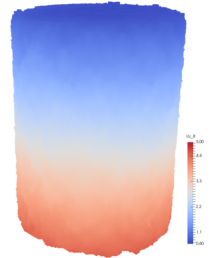
\includegraphics[width=0.4\textwidth]{DVC/deplacement_resized.png}}
			\hfill
			\subfloat[Déformation axiale]{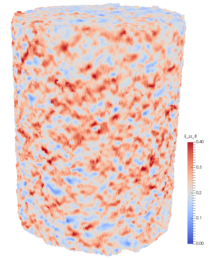
\includegraphics[width=0.4\textwidth]{DVC/deformation_resized.png}}\hfill~
			\caption{\label{fig04:champ_deplacement_deformation}Champs de déplacement axial (a) et de de déformation axiale (b) de l'échantillon dont la pression de confinement est de \SI{1}{\mega\pascal} pour le dernier état de compression.}
		\end{figure}
		\\Deux méthodes d'analyse des déformations ont été considérées. Dans un premier temps, les déformations sont calculées entre chaque états de compression successifs, en considérant le premier état comme géométrie de référence. Dans un second temps, les déformations sont calculées entre chaque états de compression et l'état non déformé. Les résultats présentés ci-après sont ceux issus de la seconde méthode.
		\\Puisque l'ensemble des composantes du tenseur des déformations est connu, il est possible de définir la partie sphérique $\doubleunderline{\varepsilon_v}$ du tenseur $\doubleunderline{\varepsilon}$ pour établir les déformations déviatoires $\doubleunderline{\varepsilon_d}$ et ainsi connaître localement les déformations volumique $\varepsilon_v$ et déviatoire $\varepsilon_d$. Pour rappel (cf. formule (\ref{eq03:decomposition_defo_triax})), si $\doubleunderline{\varepsilon}$ est le tenseur des déformations calculé entre deux états de compression successifs (le tenseur de Green-Lagrange linéarisé est alors considéré) alors les déformations volumique et déviatoire pour un essai de compression triaxiale peuvent être définies par :
		\begin{equation}\label{eq04:defo_deviatoire_volumique}
			\varepsilon_v = \mathrm{tr} \left( \doubleunderline{\varepsilon} \right)
			\qquad\text{et}\qquad
			\varepsilon_d = \sqrt{\cfrac{2}{3}\;\mathrm{tr}(\doubleunderline{\varepsilon_d}^2)}
		\end{equation}
		\\Puisque les déformations sont calculées à partir d'une grille régulière des déplacements, chacune des composantes du tenseur des déformations défini dans (\ref{eq04:defo_DVC}) est également représentée dans l'espace par cette même grille régulière. Une carte des déformations est ainsi créée (figure \ref{fig04:champ_deplacement_deformation}-(b)). Dans toute cette partie, la déformation volumique associée à un état de compression est considérée positive, au contraire, elle est négative lorsque le volume final est supérieur au volume initial.
		\paragraph{}
		Une méthode d'analyse de la déformation globale de l'échantillon en cours de chargement consiste à considérer la valeur moyenne du champ de déformation dans l'échantillon. Les courbes de la figure \ref{fig04:global_defo_vol_dev} permettent de visualiser l'évolution des valeurs ainsi mesurées pour les déformations volumique et déviatoire en fonction de la déformation axiale de chacun des échantillons. La figure \ref{fig04:global_defo_vol_dev}-(a) peut être analysée de la même manière que la figure \ref{fig04:bulkDensities} puisque l'étude de la déformation volumique et intimement liée à celle de la densité. Il est observé, en effet, que l'échantillon dont la pression de confinement est la plus élevée (\SI{7}{\mega\pascal}) ne cesse de se densifier tout au long de l'essai. Pour la pression de confinement de \SI{2}{\mega\pascal}, la densification de l'échantillon est stoppée pour les plus grandes déformations axiales. Enfin, la pression de confinement de \SI{1}{\mega\pascal} engendre un effet de dilatance à partir du milieu du chargement axial. Pour cette pression de confinement, l'échantillon est moins dense à l'état final qu'à l'état avec la seule pression de confinement, bien qu'il reste plus dense que l'état naturel. Encore une fois, il est remarqué que la pression de confinement joue un rôle important dans la densification de l'échantillon. L'augmentation de la pression de confinement a un effet "rigidifiant" sur l'échantillon et favorise la déformation des grains ductiles en dépit du glissement, la probabilité d'observer des phénomènes de dilatance et de bandes de cisaillement en est donc également minimisée.
		Ce dernier point est vérifié sur la figure \ref{fig04:global_defo_vol_dev}-(b). En effet, les courbes indiquent que les déformations liées au cisaillement, pour une même déformation axiale, sont inversement proportionnelles à la pression de confinement. De manière évidente, il est également observé l'absence de déformations déviatoires lors des étapes de confinement (chargement isotrope).
		\begin{figure}\centering
			\subfloat[]{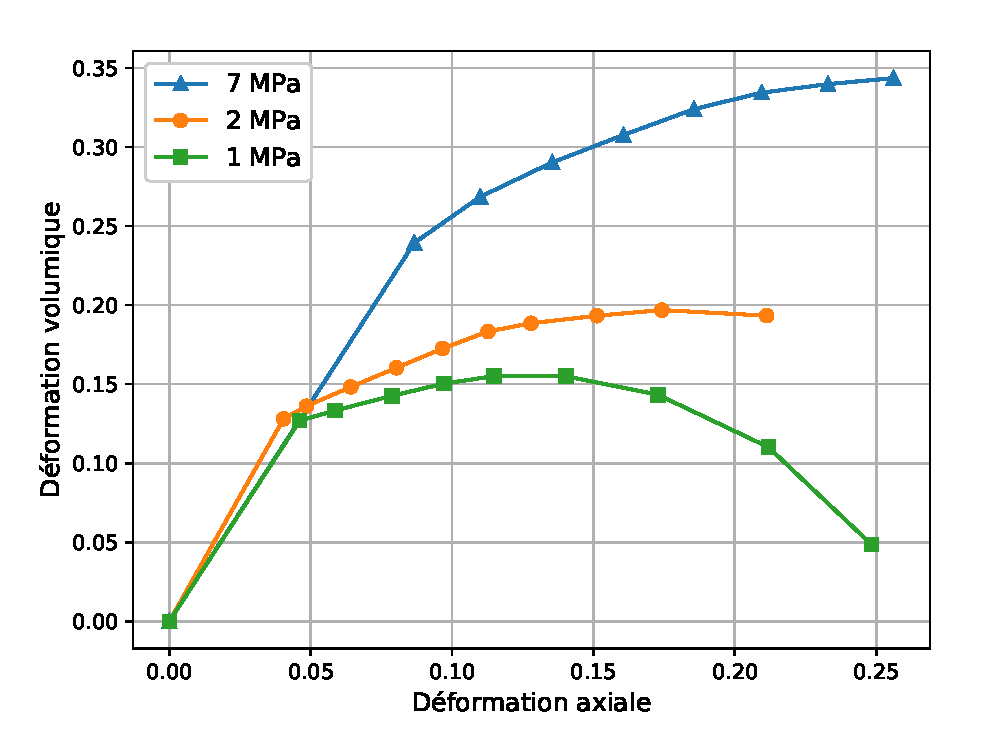
\includegraphics[width=0.48\textwidth]{global_strains/global_volumetric.eps}}
			\hfill
			\subfloat[]{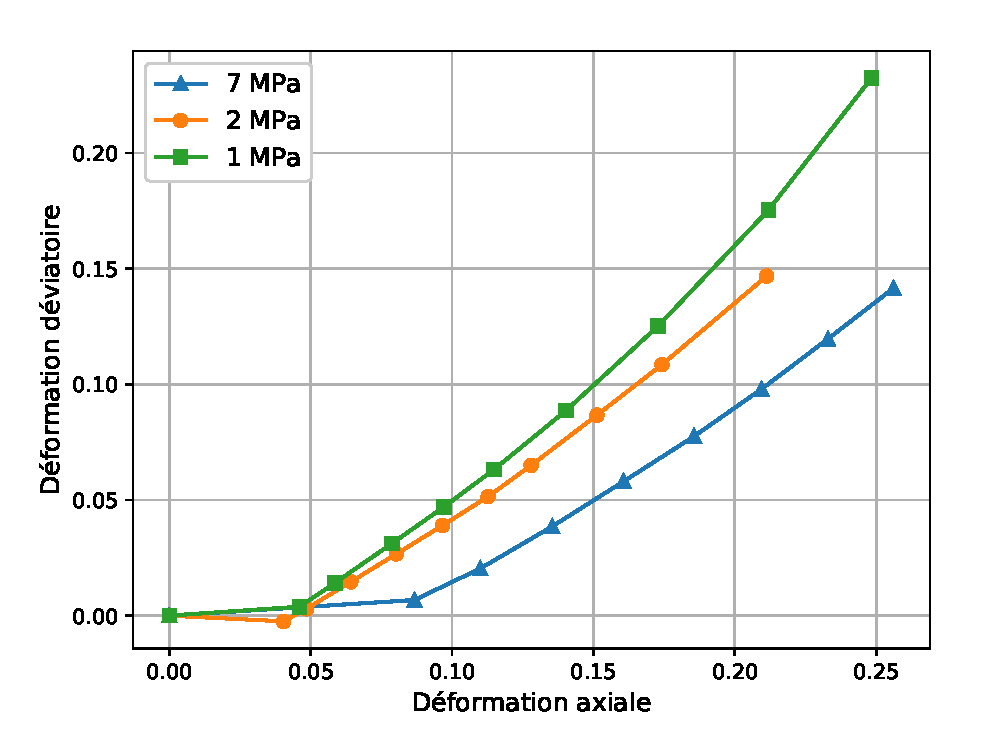
\includegraphics[width=0.48\textwidth]{global_strains/global_deviatoric.eps}}
			\caption{\label{fig04:global_defo_vol_dev}Déformations (a) volumique $\varepsilon_v$ et (b) déviatoire $\varepsilon_d$ moyennées de l'ensemble des échantillons par rapport à la déformation axiale.}
		\end{figure}
		\paragraph{}
		Comme il l'a déjà été expliqué avec l'analyse de la densité, l'étude locale des déformations présente également un certain intérêt. En effet, l'étude multi-échelle des champs de densité et déformation permet une analyse plus profonde du problème.
		\begin{figure}\centering
			\subfloat[$E_C$ - Déformation volumique]{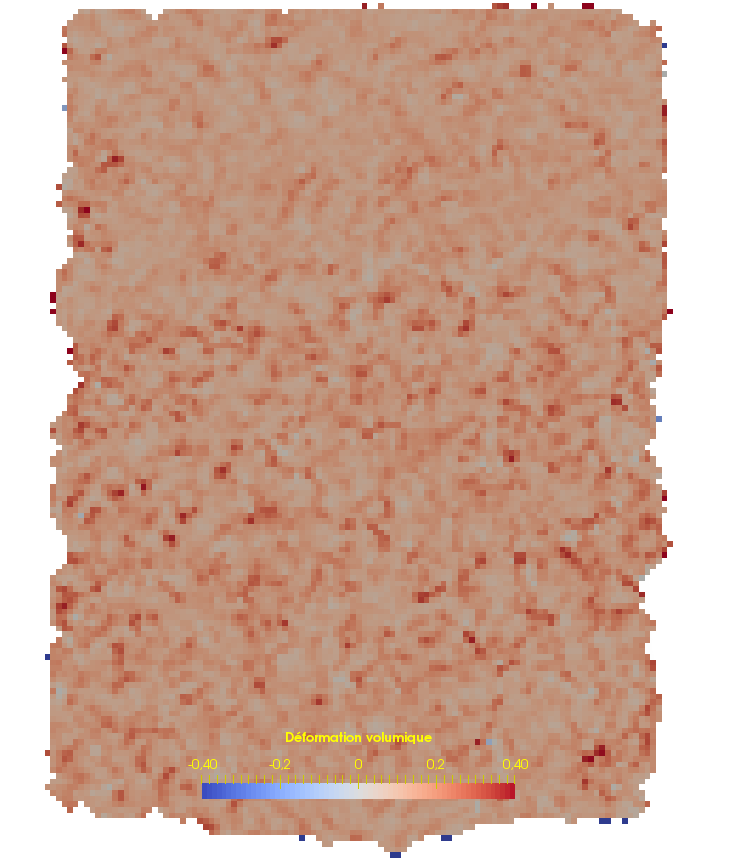
\includegraphics[width=0.49\textwidth]{local_strains/1_e_vol_0Pc.png}}
			\hfill
			\subfloat[$E_F$ - Déformation volumique]{\includegraphics[width=0.49\textwidth]{local_strains/1_e_vol_8.png}}
			\\
			\subfloat[$E_C$ - Déformation déviatoire]{\includegraphics[width=0.49\textwidth]{local_strains/1_e_dev_0Pc.png}}
			\hfill
			\subfloat[$E_F$ - Déformation déviatoire]{\includegraphics[width=0.49\textwidth]{local_strains/1_e_dev_8.png}}
			\caption{\label{fig04:champs_deformations} Déformations volumiques (a-b) et déviatoires (c-d) sur une coupe de l'échantillon dont la pression de confinement est de \SI{1}{\mega\pascal} et pour les état de compression en confinement $E_C$ (a, c) et final $E_F$ (b, d). Les cartes de couleur vont de \num{-0.4} (bleu) à \num{0.4} (rouge) pour la déformation volumique et de \num{0} (bleu) à \num{0.5} (rouge) pour la déformation déviatoire.}
		\end{figure}
		\\La figure \ref{fig04:champs_deformations} montre les mesures locales des déformations volumique et déviatoire sur une coupe (suivant la hauteur de l'échantillon et prise en son milieu) de l'échantillon dont la pression de confinement est de \SI{1}{\mega\pascal}. Deux états de compression sont représentés : l'état de confinement isotrope (sans chargement axial) et l'état final de chargement. L'étude de l'état de compression isotrope montre des champs de déformation homogènes, pour lesquels la déformation déviatoire semble être nulle en moyenne (ce qui est observé sur le figure \ref{fig04:global_defo_vol_dev}-(b)) et la déformation volumique supérieure à \num{0} (densification liée au confinement). L'analyse de l'état de compression finale est toute autre. Les champs de déformation ne sont plus homogènes et il est observé l'apparition de zones de fort cisaillement (zones en rouge sur la figure \ref{fig04:champs_deformations}-(d)). La figure \ref{fig04:champs_deformations}-(b), qui permet d'observer localement si la densification est positive (toutes les nuances de rouge) ou négative (toutes les nuances de bleu), présente les mêmes zones. Les zones de l'échantillon pour lesquelles la déformation déviatoire est la plus grande (en rouge sur la figure \ref{fig04:champs_deformations}-(d)) voient leur volume augmenter sous l'effet de la dilatance, d'où une déformation volumique négative (zones bleues sur la figure \ref{fig04:champs_deformations}-(b)). L'agencement des zones concernées par cet effet sur les figures \ref{fig04:champs_deformations}-(b) et (d) laisse supposer l'apparition d'une bande de cisaillement en cours de développement. C'est autour de cette bande que le phénomène de dilatance est le plus marqué.
		\\Finalement, l'analyse locale de la déformation permet de confirmer et expliquer les résultats observés lors de l'étude globale de la déformation de l'échantillon.
		\begin{figure}[]\centering
			\subfloat[$E_C$ - Déformation volumique]{\includegraphics[width=0.49\textwidth]{local_strains/2_e_vol_0Pc.png}}
			\hfill
			\subfloat[$E_F$ - Déformation volumique]{\includegraphics[width=0.49\textwidth]{local_strains/2_e_vol_9.png}}
			\caption{\label{fig04:champs_deformations_2MPa} Déformations volumiques sur une coupe de l'échantillon dont la pression de confinement est de \SI{2}{\mega\pascal} et pour les état de compression en confinement $E_C$ (a) et final $E_F$ (b). Les cartes de couleur indiquent la déformation volumique et vont de \num{-0.4} (bleu) à \num{0.4} (rouge).}
		\end{figure}
		\begin{figure}[h]\centering
			\subfloat[$E_C$ - Déformation volumique]{\includegraphics[width=0.49\textwidth]{local_strains/7_e_vol_0Pc.png}}
			\hfill
			\subfloat[$E_F$ - Déformation volumique]{\includegraphics[width=0.49\textwidth]{local_strains/7_e_vol_7.png}}
			\caption{\label{fig04:champs_deformations_7MPa} Déformations volumiques sur une coupe de l'échantillon dont la pression de confinement est de \SI{7}{\mega\pascal} et pour les état de compression en confinement $E_C$ (a) et final $E_F$ (b). Les cartes de couleur indiquent la déformation volumique et vont de \num{-0.6} (bleu) à \num{0.6} (rouge).}
		\end{figure}
		\\L'analyse des échantillons dont la pression de confinement est plus grande (\num{2} et \SI{7}{\mega\pascal}) rend compte d'une hétérogénéité des déformations moins marquée. Ce résultat est observable sur les figures \ref{fig04:champs_deformations_2MPa} (confinement de \SI{2}{\mega\pascal}) et \ref{fig04:champs_deformations_7MPa} (confinement de \SI{7}{\mega\pascal}). Contrairement à l'échantillon subissant une pression de confinement de \SI{1}{\mega\pascal}, ces deux échantillons ne présentent presque aucune zone dont la déformation volumique est négative (zones bleues). Cela veut dire que la densification de la poudre se réalise tout au long du chargement et en tout point des échantillons. La variation de contraste des champs de déformation entre les différents états de compression est faible : cela montre en plus que la déformation est relativement homogène lorsque la pression de confinement est suffisamment grande. Ce résultat montre encore une fois que les grains ont plus de difficulté à glisser les uns par rapport aux autres lorsque la pression de confinement est grande. C'est la raison pour laquelle le phénomène de dilatance n'est pas observé dans ces deux figures : les grains se déforment suffisamment pour ne pas avoir à glisser les uns par rapport aux autres.
		